\section{Ergebnisse}

Unsere Studie wurde vom 04. Juni bis zum 18. August 2019 durchgeführt. Es nahmen insgesamt 45 Teilnehmer in zwei Durchläufen teil. Der erste Durchlauf erfasste zwei Gruppen, dessen geänderter Parameter die Zeit war, in der ein Licht innerhalb der virtuellen Umgebung die Probanden 'geweckt' hat. Im zweiten Durchlauf wurde dieser Parameter geändert und die Teilnehmer wurden mit einem Ton geweckt, wie man ihn als Hinweiston in modernen Autos wiederfindet. Hierbei wurde die Zeit, in der die Studienteilnehmer den Ton selbständig abgeschaltet haben gemessen. Zusätzlich zur Interaktionen zwischen Proband und VR System wurden noch einige demografische und personenbezogene Fragen außerhalb der VR Umgebung gestellt, welche zusätzlich aufgelistet werden.

\subsection{Demografische Ergebnisse}

Es waren von den 45 Teilnehmern nach eigenen Angaben 12 weiblich, 33 männlich und 0 Divers. Eine grafische Repräsentation kann in Abbildung~\ref{fig:gender} und die zugehörigen Zahlenwerte in Tabelle~\ref{tab:sc_results_gender} eingesehen werden. Die Teilnehmer haben eine große Bandbreite an Studiengängen abgedeckt, welche neben diversen Naturwissenschaften auch beispielsweise Informatik, Wirtschaftsmathematik und Psychologie beinhalteten. Diese können in Tabelle~\ref{tab:sc_results_study} entnommen werden können.

\begin{figure}[H]
	\centering
	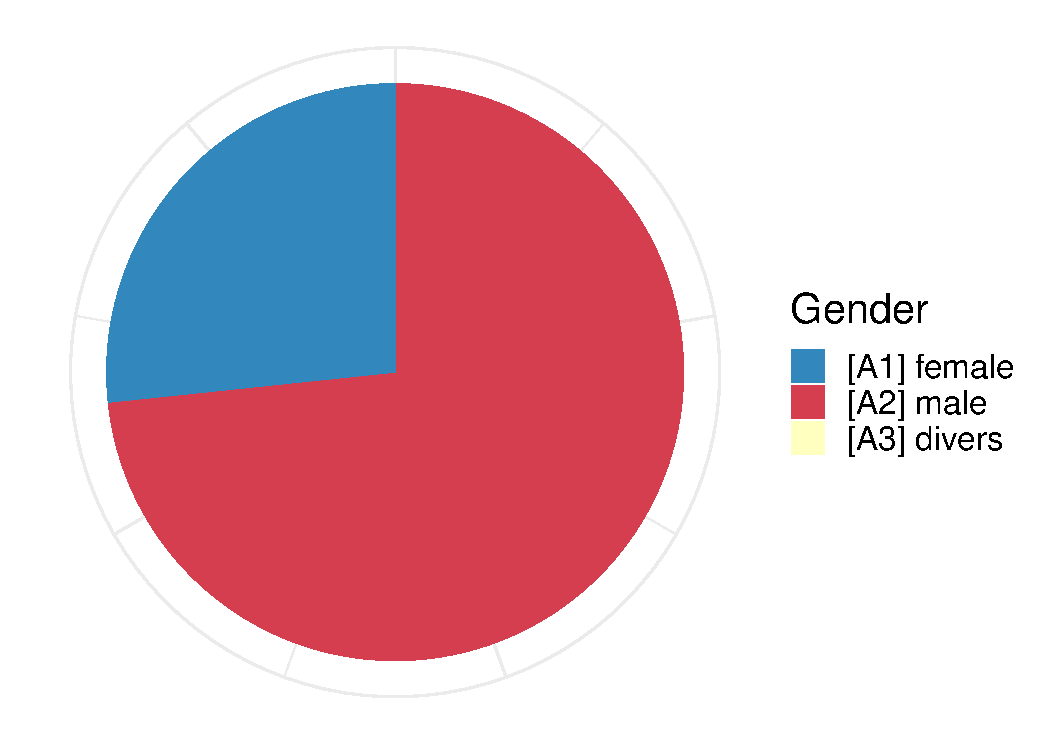
\includegraphics[width=0.75\textwidth]{./_StudyResults/gender}
	\caption{Geschlechterverteilung der Studienteilnehmer}
	\label{fig:gender}
\end{figure}

Das Alter der Teilnehmer reichte von 19 bis 30 Jahren, wobei der Median bei 23 und der Mittelwert bei 23,04 Jahren mit einer Standardabweichung von 2.53 lag. Eine grafische Darstellung kann in Abbildung~\ref{fig:age} und die zugehörigen Zahlenwerte in Tabelle~\ref{tab:sc_results_age} gesehen werden.

\begin{figure}[H]
	\centering
	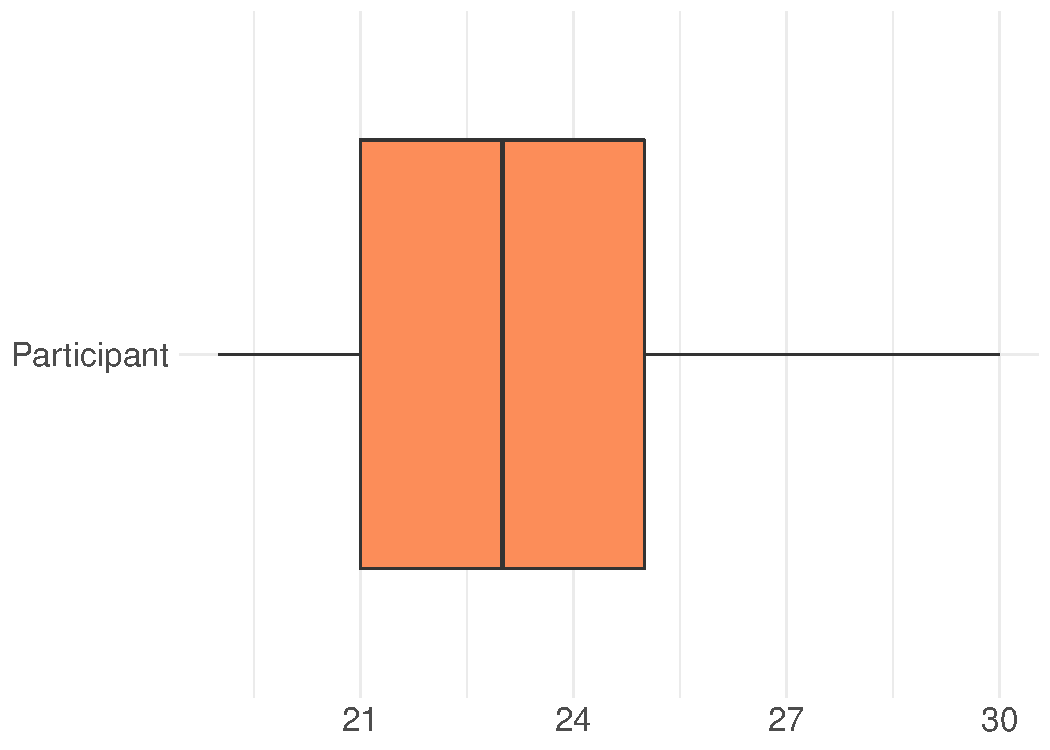
\includegraphics[width=0.75\textwidth]{./_StudyResults/age}
	\caption{Boxplot des Alters der Studienteilnehmer}
	\label{fig:age}
\end{figure}

Die Teilnehmer gaben an, dass sie unterdurchschnittlich wenig Erfahrung mit virtueller Realität haben. Hierbei lag der Mittelwert bei 2,93 von 7 möglichen Punkten. Die Standardabweichung beträgt 1,78. Die Ergebnisse können auch in Tabelle~\ref{tab:sc_results_expVR} und Tabelle~\ref{tab:sc_numbers_expVR} angesehen werden. Bei augmentierter Realität sehen wir ein ähnliches Abbildung. Hier gaben die Teilnehmer an einen durchschnittlichen Erfahrungswert von 2.36 von 7 zu haben. Die Standardabweichung in diesem Fall beträgt 1,38. Außerdem ist noch hervorzuheben, dass keiner der Befragten einen Wert von 7 ausgewählt hat. Die Ergebnisse hierzu können in Tabelle~\ref{tab:sc_results_expAR} und Tabelle~\ref{tab:sc_numbers_expAR} eingesehen werden, zusätzlich existiert eine grafische Repräsentation in den Abbildungen~\ref{fig:expVr} und~\ref{fig:expAr}.

\begin{figure}[H]
	\centering
	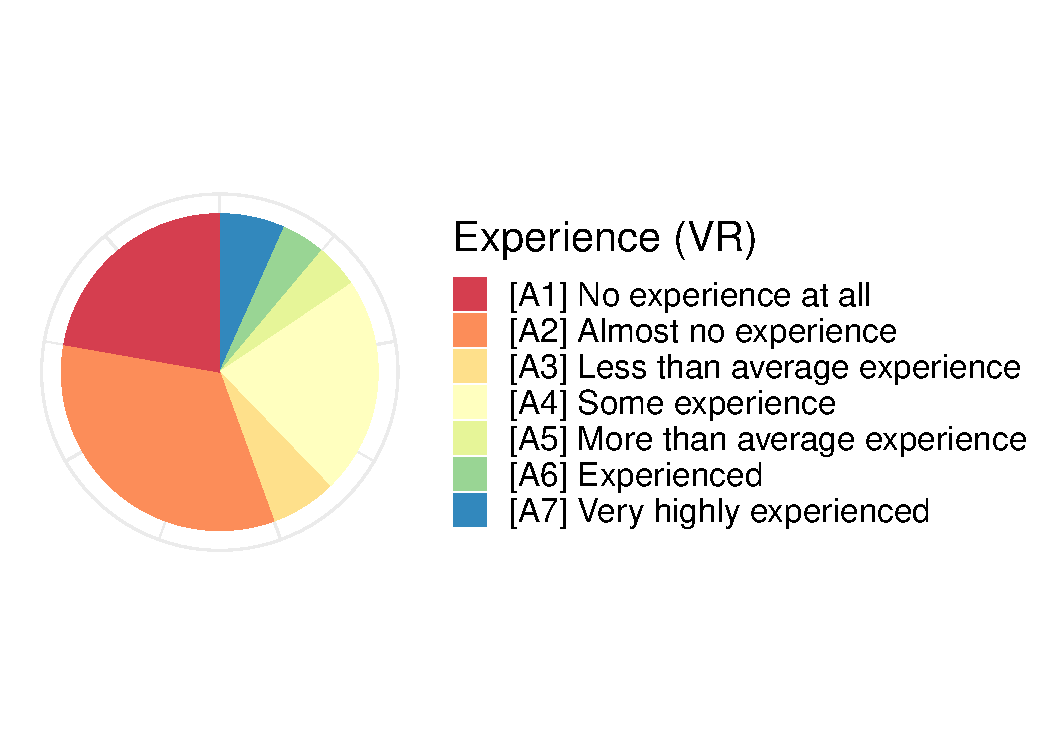
\includegraphics[width=0.75\textwidth]{./_StudyResults/expVr}
	\caption{Grafische Repräsentation der Antworten zur Frage "`How much experience do you have with VR?"'.}
	\label{fig:expVr}
\end{figure}%
\begin{figure}[H]
	\centering
	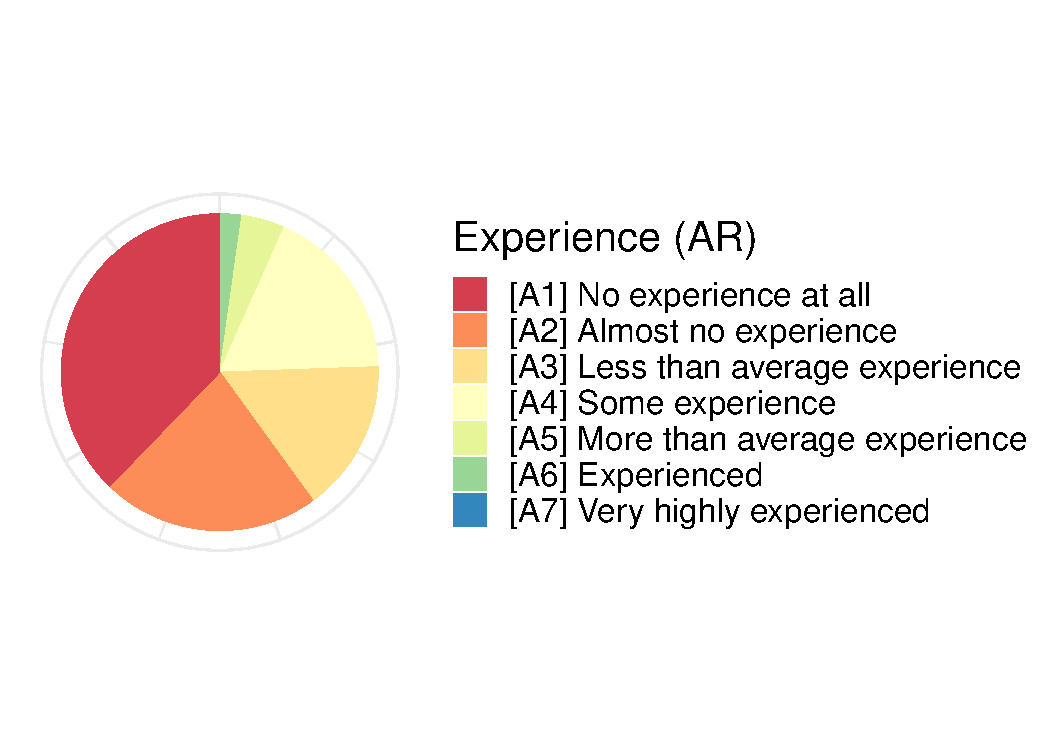
\includegraphics[width=0.75\textwidth]{./_StudyResults/expAr}
	\caption{Grafische Repräsentation der Antworten zur Frage "`How much experience do you have with AR?"'.}
	\label{fig:expAr}
\end{figure}

\subsection{Umgebungsvariablen}
\subsubsection{Stuhleinstellungen}

Die Umgebung der Studie wurde so abgeschottet gewählt, dass wenig äußere Einflüsse störend auf den Studienablauf wirken konnten. Trotz dieser Platzwahl bekamen wir Rückmeldung durch die Probanden, dass sie die Umgebung nicht perfekt zum Einschlafen gewählt wurde. Weitere Kommentare der Nutzer zur Bequemlichkeit der VR Brille, als auch zum Stuhl, sowie allen weiteren Umgebungsvariablen können im Anhang gefunden werden.

Die durchschnittliche Neigung der Stuhllehne lag über alle Durchläufe bei 38,6$^\circ$. Eine genaue Auflistung der Einstellungen kann in Tabelle~\ref{tab:sc_results_chair} eingesehen werden. Hierbei ist zu beachten, dass die Werte vom Studienbetreuer zur Zeit der Ruhephase subjektiv notiert wurden. Außerdem ist zu beachten, dass die Winkeleinstellung mit einer Abweichung notiert worden sein kann. Hierdurch ergeben sich die hier aufgeführten Ergebnisse. Die möglichen Einstellung des verwendeten Stuhls können in Abbildung~\ref{fig:chair_backrest} gefunden werden.

\begin{figure}[H]
	\centering
	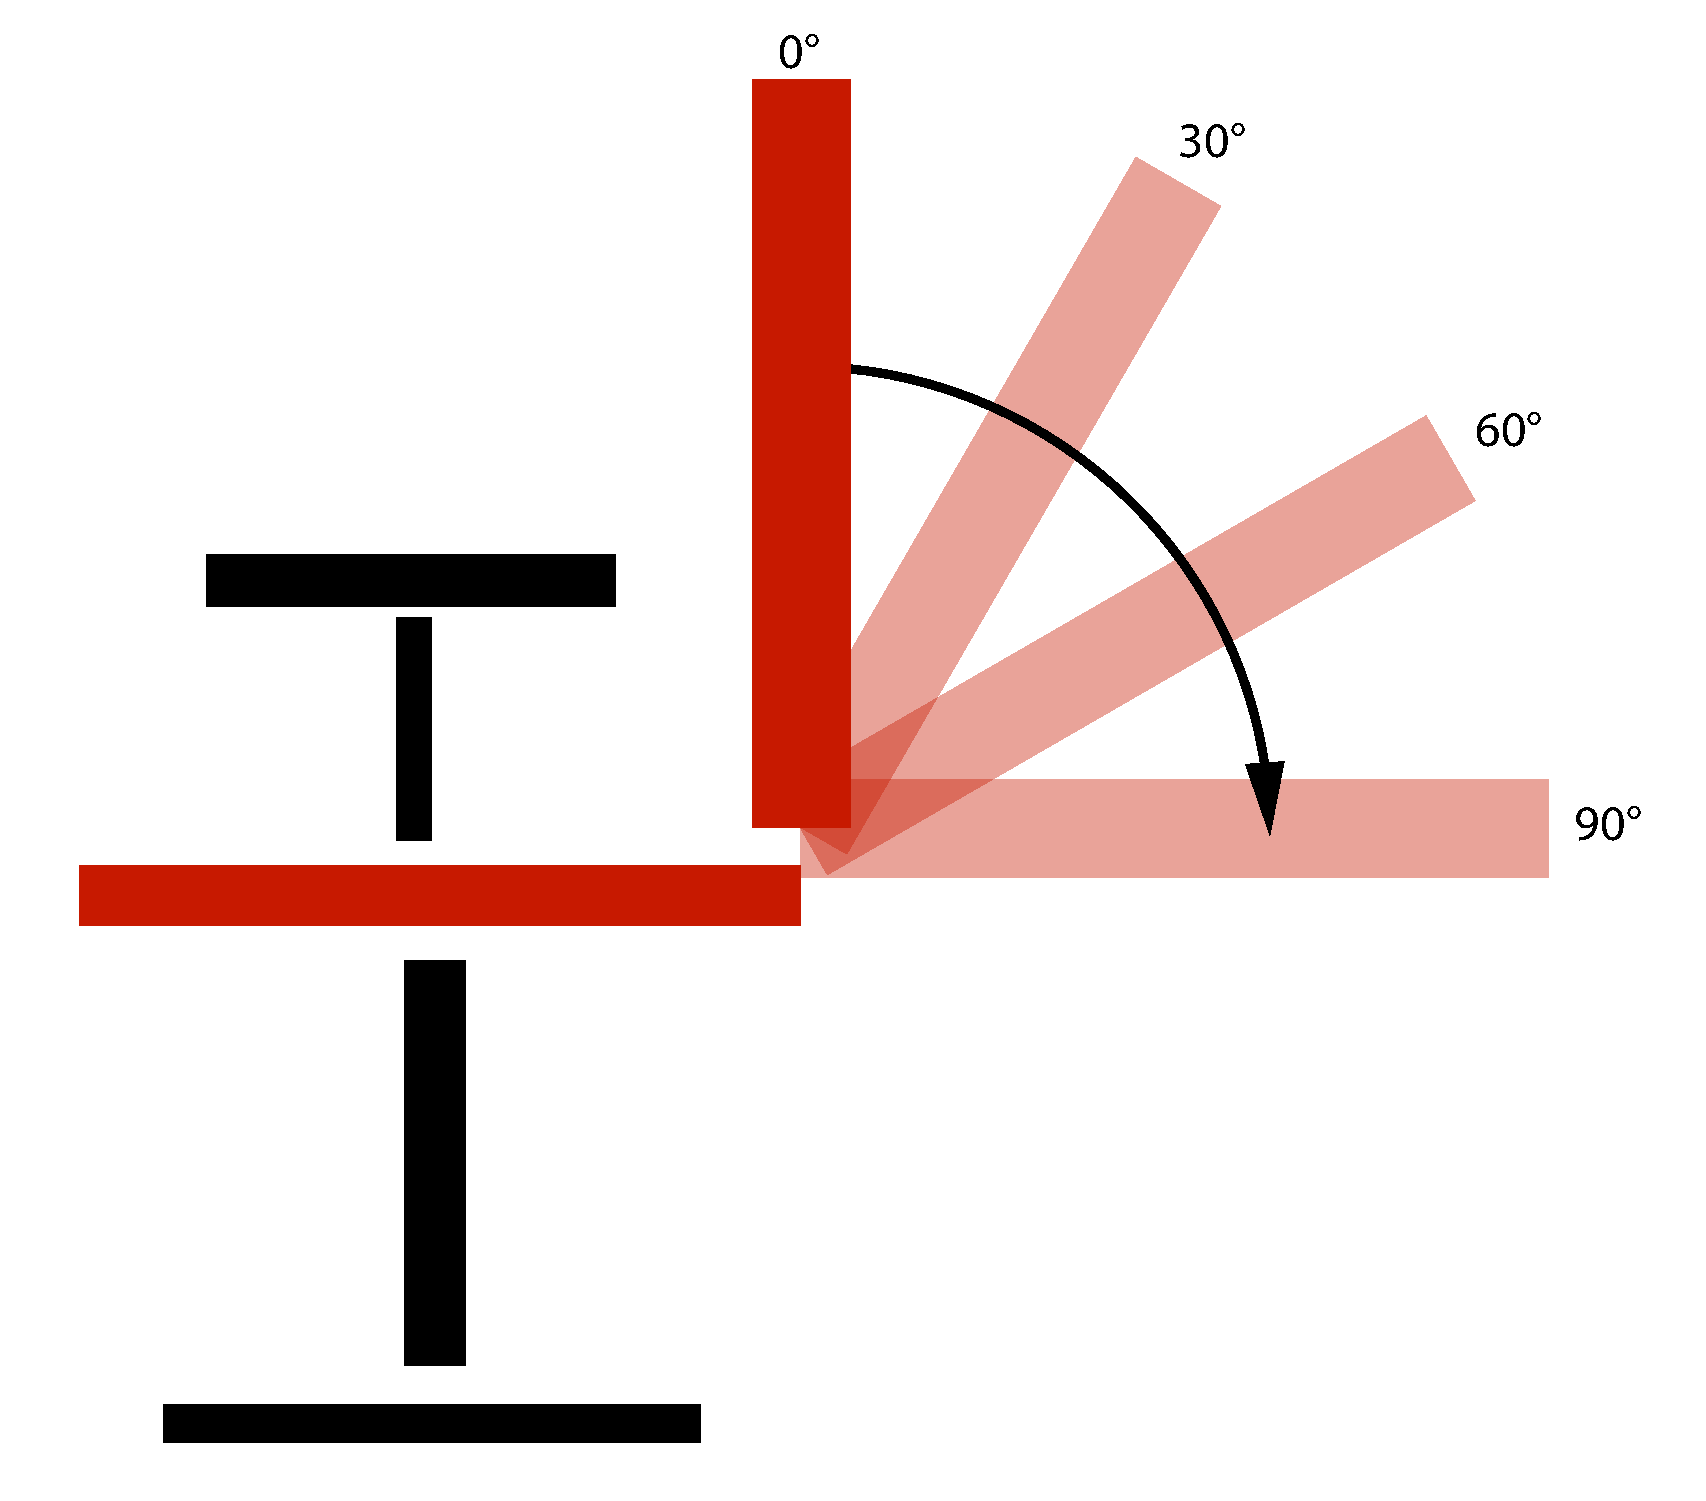
\includegraphics[width=0.75\textwidth]{./images/chair}
	\caption{Winkeleinstellungen vom verwendeten Stuhl in der Studie}
	\label{fig:chair_backrest}
\end{figure}


\subsubsection{Dauer des Wecker-Tons}

Die Probanden die mit Ton geweckt wurden, hatten einen Button der den Aufwachteil der Zeitmessung beendet hat. Diese Zeiten reichten von 3.91 bis 10.84 Sekunden. Der Median des Ton-Abstellens beträgt 5.87 Sekunden, also betätigten die meisten Teilnehmer ca. nach 6 Sekunden den Button der sie zur ersten Aufgaben weitergeleitet hat. 

\begin{figure}[H]
	\centering
	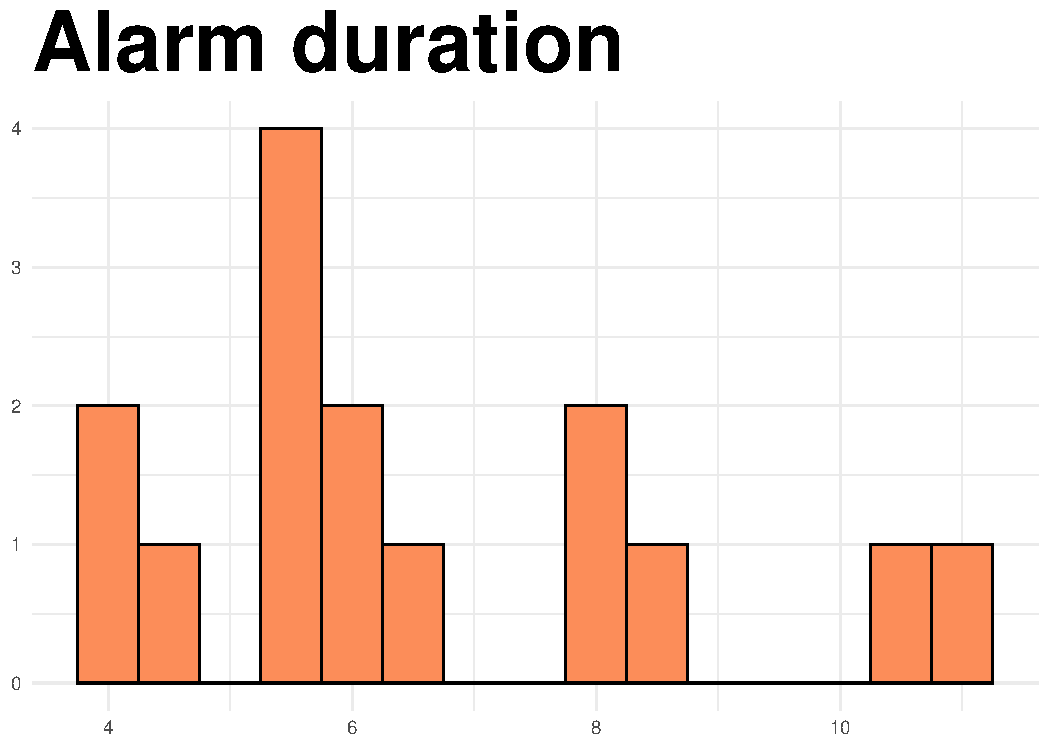
\includegraphics[width=0.75\textwidth]{./_StudyResults/alarmDurationHist}
	\caption{Histogramm der Zeit (s), wie lange die Teilnehmer der Studie den Wecker-Ton laufen ließen. Genauigkeit: 500ms}
	\label{fig:alarmDurationHist}
\end{figure}

\subsection{Aufgabenergebnisse} 

Ein Hauptaspekt der Studie liegt auf der Aufgabenbewältigung und vor allem darauf, wie gut diese gelöst werden können unter den uns bekannten Einflüssen. 

\subsubsection{Fehlerraten}

Die Unterteilung in unsere 3 Gruppen, die wir untersucht haben, lässt sich im Folgenden so verstehen, dass die Gruppe \textit{Fade 5}, die Gruppe mit 5 FadeSeconds beim Aufwachen ist und die zweite Gruppe \textit{Fade 20} die mit 20 Sekunden FadeSeconds ist. Als dritte Studiengruppe haben wir die Gruppe \textit{Alarm}, bei welcher die Probanden durch den Weckton geweckt wurde.

Für die erste Aufgabe gilt, dass ein Fehler dann als Fehler gewertet wird, wenn danach eine kleinere Zahl vorkommt. Eine ausgewählte Reihenfolge $3, 2, 1$ zählt also als 3 Fehler insgesamt, da $3 > 2 > 1$ (2 Fehler) sowie $2 > 1$ (1 Fehler). Auf diese Weise kommen auch 45 Fehler zustande; und zwar dann, wenn alle Zahlen falsch herum ausgewählt wurden. Dies entspricht der Summe von 1 bis 9.
Wie in Tabelle~\ref{fig:orderingMistakeHistogram} abzulesen, haben nur knapp 58\% der Studienteilnehmer überhaupt keine Fehler begangen. Häufig wurden vereinzelte Fehler gemacht, welche die Teilnehmer direkt beim Ausführen der Aufgabe bemerkten, was meist durch verbale oder physische Reaktionen deutlich wurde. 
Eine Fehlerzahl von 44 oder 45 wurde dann erreicht, wenn die Probanden gedacht haben, sie sollen die Zahlen genau andersherum sortieren, wie uns im Nachhinein mehrere Nutzer mitgeteilt haben.
Aus der Gruppe Fade 5 haben am Meisten mit 0 Fehlern abgeschnitten. Die schlechtesten Ergebnisse stammen aus der Alarm Gruppe, wie in Abbildung~\ref{fig:orderingMistakeHistogram} erkennbar ist. \todoAll{mehr Fehler Aufg 1 beschreiben?}

\begin{figure}[H]
	\centering
	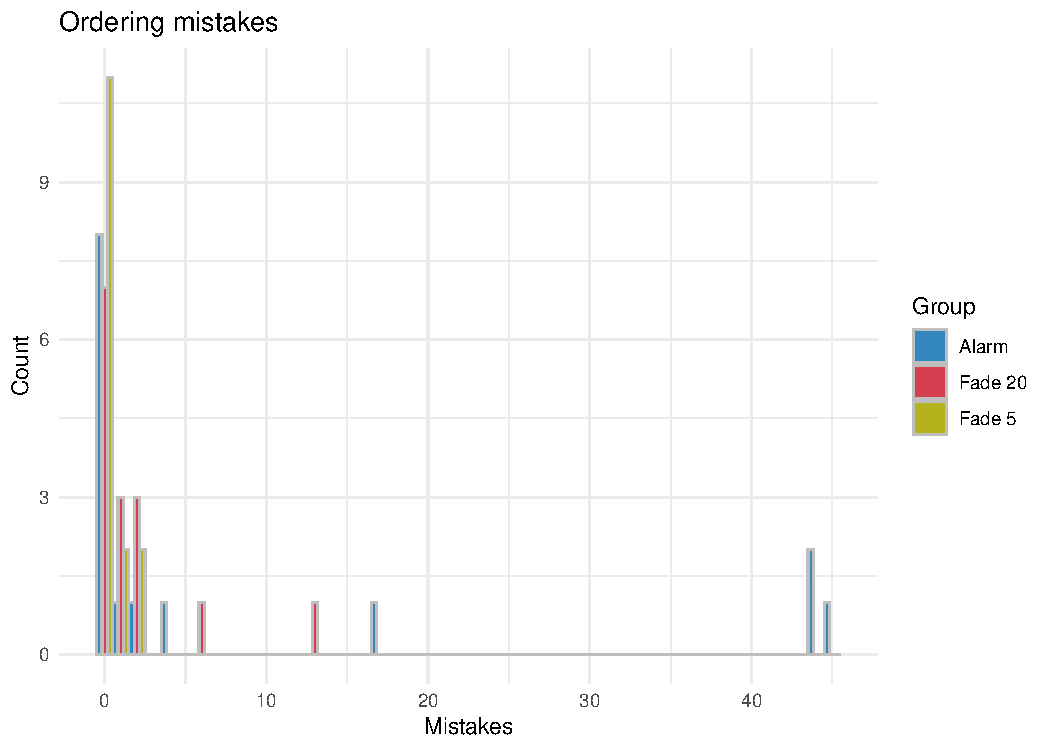
\includegraphics[width=0.75\textwidth]{./_StudyResults/orderingMisHist}
	\caption{Häufigkeit der Fehler unterteilt in Gruppen in Aufgabe 1: Zahlenfolge. Darstellungsgenauigkeit: 1}
	\label{fig:orderingMistakeHistogram}
\end{figure}

\begin{table*}
	\caption{Vorkommnisse der Fehler unterteilt in Gruppen in Aufgabe 1: Zahlenfolge.}~\label{tab:orderingMistakeNumbers}
	
	\setlength\tabcolsep{3pt}
	\renewcommand{\arraystretch}{1.4}% for the vertical padding
	\begin{tabularx}{\textwidth}{ | l | x | x | x | x | x | x | x | x | x | }
		\hline
		Anzahl Fehler & 0   & 1  & 2  & 4  & 6  & 13 & 17 & 44  & 45 \\ \hline\hline
		Alarm 	  & 8  & 1  & 1  & 1  & 0  & 0  & 1  &  2  & 1  \\ \hline
		Fade 20	  & 7  & 3  & 3  & 0  & 1  & 1  & 0  &  0  & 0  \\ \hline
		Fade 5	  & 11  & 2  & 2  & 0  & 0  & 0  & 0  &  0  & 0  \\ \hline
	\end{tabularx}
\end{table*}

In Aufgabe 2 ist ein Fehler dann gegeben, wenn das ausgewählte Feld nicht dem gefordertem Feld entspricht, also ist das Maximum 10.
Von ca 73\% wurde diese Aufgabe komplett fehlerfrei gelöst.
Auch hier wurden Fehlerzahlen die 8 oder höher waren dann erzielt, wenn die Aufgabe so verstanden wurde, dass die Farbe in der das Wort geschrieben stand gewählt wurde.
Aus Abbildung~\ref{fig:matchingMistakeHistogram} ist deutlich ablesbar, dass aus den Gruppen Alarm und Fade 5 gleich viele Fehler gemacht haben. Bis auf ein paar Probanden die die Aufgabe nicht komplett richtig bearbeitet haben weißt die dritte Gruppe Fade 20 keine Unterschiede auf.

\todoTob{nicht gut ablesbar, wo die Blaken dazugehören, also bspw zweiter roter von links hat der mit dem blauen daneben zu tun oder nicht? vielleicht so kleine schwarze striche an der x achse die zeigen hier ist ein schritt? Und bei mistakes steht bei der x achse 2.5 das ist glaub verwirrend weil gibt ja keine halben fehler}

\begin{figure}[H]
	\centering
	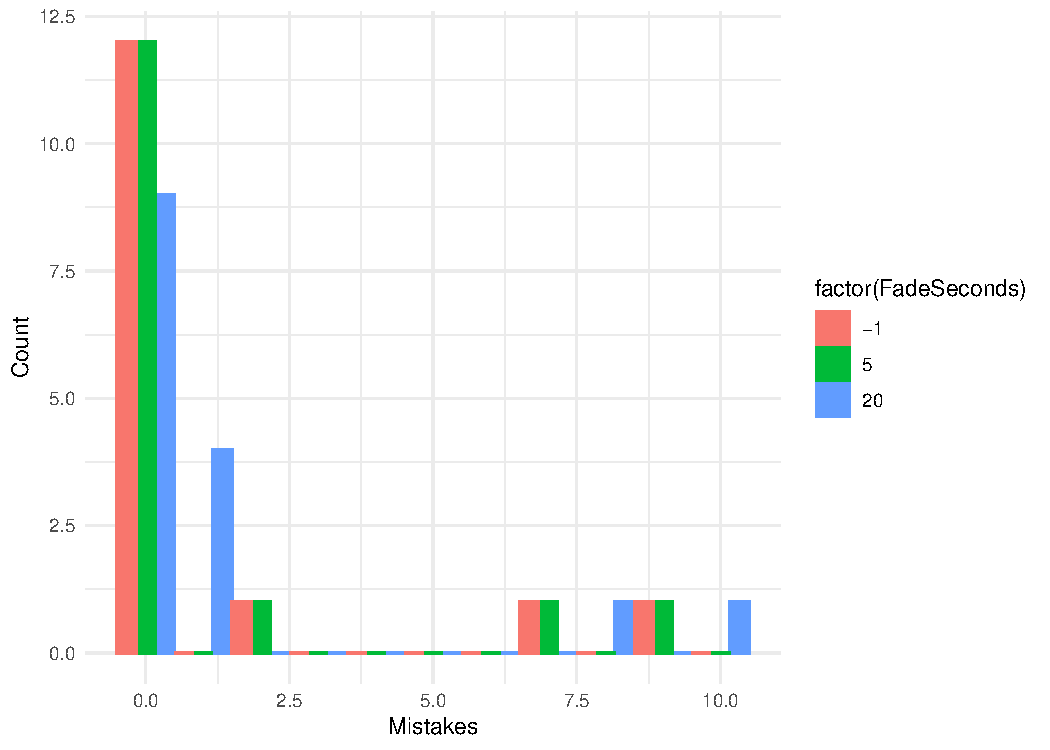
\includegraphics[width=0.75\textwidth]{./_StudyResults/matchingMisHist}
	\caption{Häufigkeit der Fehler unterteilt in Gruppen in Aufgabe 2: Stroop-Effekt. Darstellungsgenauigkeit: 1}
	\label{fig:matchingMistakeHistogram}
\end{figure}

\begin{table*}
	\caption{Vorkommnisse der Fehler unterteilt in Gruppen in Aufgabe 2: Stroop-Effekt.}~\label{tab:matchingMistakeNumbers}
	
	\setlength\tabcolsep{3pt}
	\renewcommand{\arraystretch}{1.4}% for the vertical padding
	\begin{tabularx}{\textwidth}{ | l | x | x | x | x | x | x | x | }
		\hline
		Anzahl Fehler & 0   & 1  & 2  & 7  & 8  & 9 & 10 \\ \hline\hline
		Alarm 	  & 12  & 0  & 1  & 1  & 0  & 1 & 0  \\ \hline
		Fade 20   & 9  & 4  & 0  & 0  & 1  & 0 & 1  \\ \hline
		Fade 5 	  & 12  & 0  & 1  & 1  & 0  & 1 & 0  \\ \hline
	\end{tabularx}
\end{table*}

In Aufgabe 3 zählt ein Fehler dann, wenn nicht die richtige Anzahl von den gegebenen Auswahlmöglichkeiten gewählt wurde. Die maximale Anzahl an Fehlern ist bei 3 Durchläufen also drei.
Von knapp 75\% wurde diese Aufgabe fehlerfrei gemeistert und kein Proband hat alle 3 Boxenzahlen falsch bestimmt. Die durchschnittliche Fehleranzahl beträgt 0.31, was unter Anderem im Anhang in Tabelle~\ref{tab:sc_results_counting} nachzulesen ist.
Aus Abbildung~\ref{fig:countingMistakeHistogram} ist gut erkennbar, dass die Alarm Gruppe höchstens einen Fehler gemacht hat, wohingegen die Licht Gruppen jeweils auch Probanden haben, die zwei Fehler gemacht haben. Zudem haben die Licht Gruppen beide die höchste Anzahl an Probanden, die die Aufgabe fehlerlos gelöst haben.

\begin{figure}[H]
	\centering
	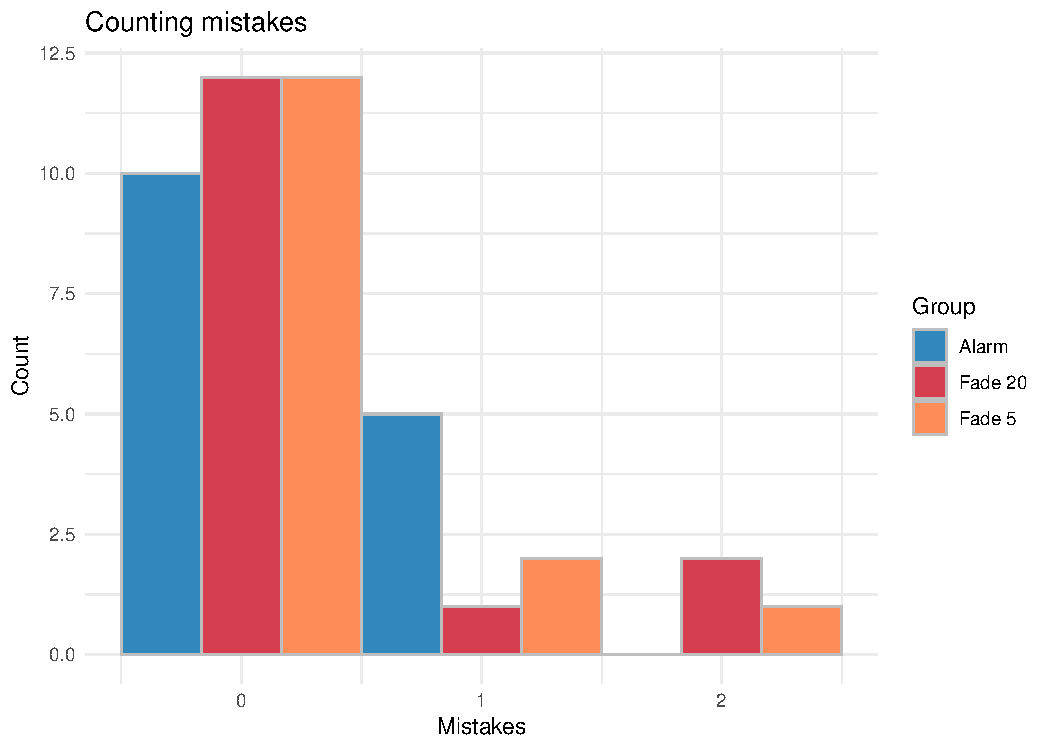
\includegraphics[width=0.75\textwidth]{./_StudyResults/countingMisHist}
	\caption{Häufigkeit der Fehler unterteilt in Gruppen in Aufgabe 3: Boxen zählen. Darstellungsgenauigkeit: 1}
	\label{fig:countingMistakeHistogram}
\end{figure}

\begin{table*}
	\caption{Vorkommnisse der Fehler in Aufgabe 3: Boxen zählen.}~\label{tab:countingMistakeNumbers}
	
	\setlength\tabcolsep{3pt}
	\renewcommand{\arraystretch}{1.4}% for the vertical padding
	\begin{tabularx}{\textwidth}{ | l | x | x | x | }
		\hline
		Anzahl Fehler & 0   & 1  & 2 \\ \hline\hline
		Alarm 	  & 10  & 5  & 0 \\ \hline
		Fade 20   & 12  & 1  & 2 \\ \hline
		Fade 5 	  & 12  & 2  & 1 \\ \hline
	\end{tabularx}
\end{table*}

\subsubsection{Benötigte Zeit für die Aufgabenerledigung}

Die jeweils gemessene Zeit erstreckt sich über den Start, der mit der Erklärung der Aufgabe gekennzeichnet wird, bis hin zum Ende der Zeitmessung, was den Abschluss der Aufgabe bedeutet.

Die Zeit, die für das Erledigen von Aufgabe 1 benötigt wurde, hat ihr Minimum bei 16.59 Sekunden. Die Anzahl der Teilnehmern die in einem Bereich von 2-Sekundenschritten, angefangen bei 15-17 Sekunden fertig geworden sind können in Abbildung~\ref{fig:orderingTimeHistogram} abgelesen werden. Die meistbenötigte Zeit 42.49 Sekunden, sowie ein Durchschnitt von 26.80 Sekunden können aus Tabelle~\ref{tab:times_results_ordering} entnommen werden.
In der Fade 5 Gruppe gibt es breit verteilte Erledigungszeiten zwischen 16 und 43 Sekunden, wohingegen sich die anderen beiden Gruppen im 20 bis 40 Sekunden Bereich aufhalten. Wie in Abbildung~\ref{fig:orderingTimeHistogram} zu erkennen ist, gibt es in der Alarm Gruppe einen Häufungspunkt bei der benötigten Zeit um die 20 Sekunden Grenze herum.

\begin{figure}[H]
	\centering
	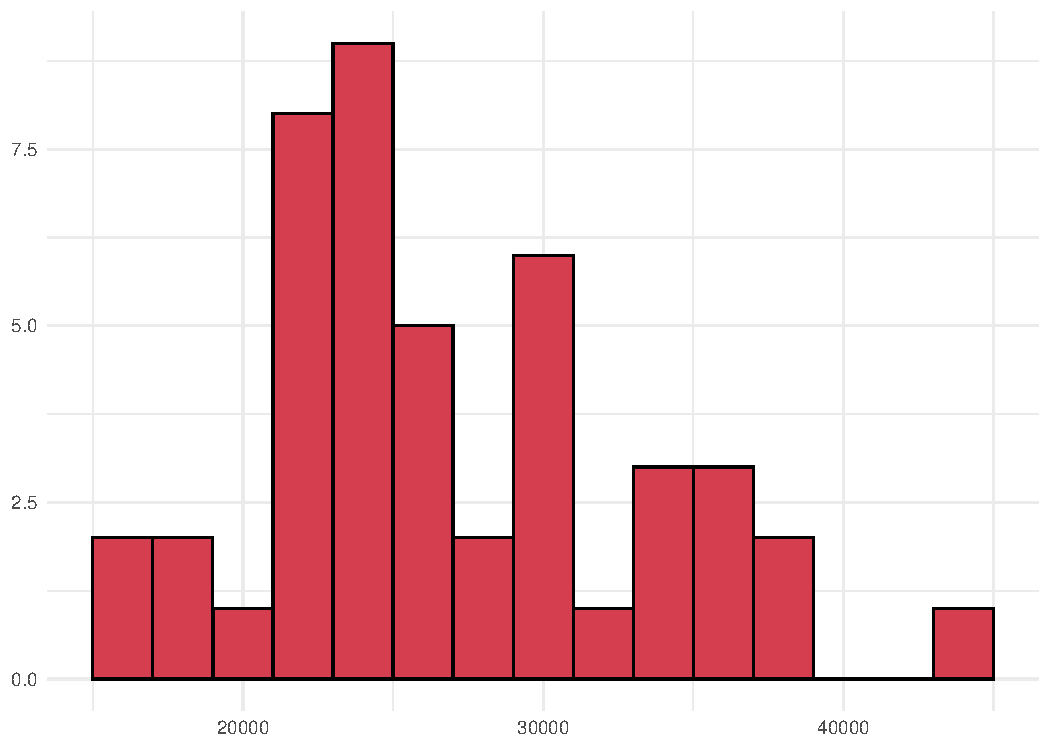
\includegraphics[width=0.75\textwidth]{./_StudyResults/orderingTimeHist}
	\caption{Histogramm der Zeit (ms) unterteilt in Gruppen zur Erledigung von Aufgabe 1: Zahlenfolge. Darstellungsgenauigkeit: 2000ms}
	\label{fig:orderingTimeHistogram}
\end{figure}

\todoTob{Median etc time für einzelne gruppen tabelle?}

Bei der zweiten Aufgabe gibt es eine größeren gemessenen Zeitbereich, was unter Anderem daran lag, dass die Probanden oft lang gebraucht haben die Aufgabenstellung zu lesen bzw. zu verstehen. Der schnellste Teilnehmer beendete die Aufgabe nach 13.87 Sekunden. Durchschnittlich haben die Probanden knapp 35 Sekunden zur Aufgabenbewältigung gebraucht. Das Maximum 83.31 Sekunden Bearbeitungszeit liegt in großem Abstand zum 'Zweitlangsamsten', welcher bei knapp unter 50 Sekunden liegt. Ein starker Häufungspunkt um die 20 Sekunden Marke kann man gut in Abbilung~\ref{fig:matchingTimeHistogram} erkennen. 
Beim Vergleich der Gruppen sieht man, dass die \textbf{XX} Gruppe im Schnitt am schnellsten mit der Bearbeitung der Aufgabe fertig war. Einzelne Teilnehmer der Fade 5 Gruppe haben länger als die Meisten gebraucht, wohingegen die Probanden aus der Fade 20 Gruppe alle zwischen 19 und 24 Sekunden gebraucht haben. Insgesamt hat die Alarm Gruppe im Vergleich zu den Licht Gruppen Teilnehmer gehabt, die alle unter 32 Sekunden zur Bewältigung der Aufgabe benötigt haben.

\begin{figure}[H]
	\centering
	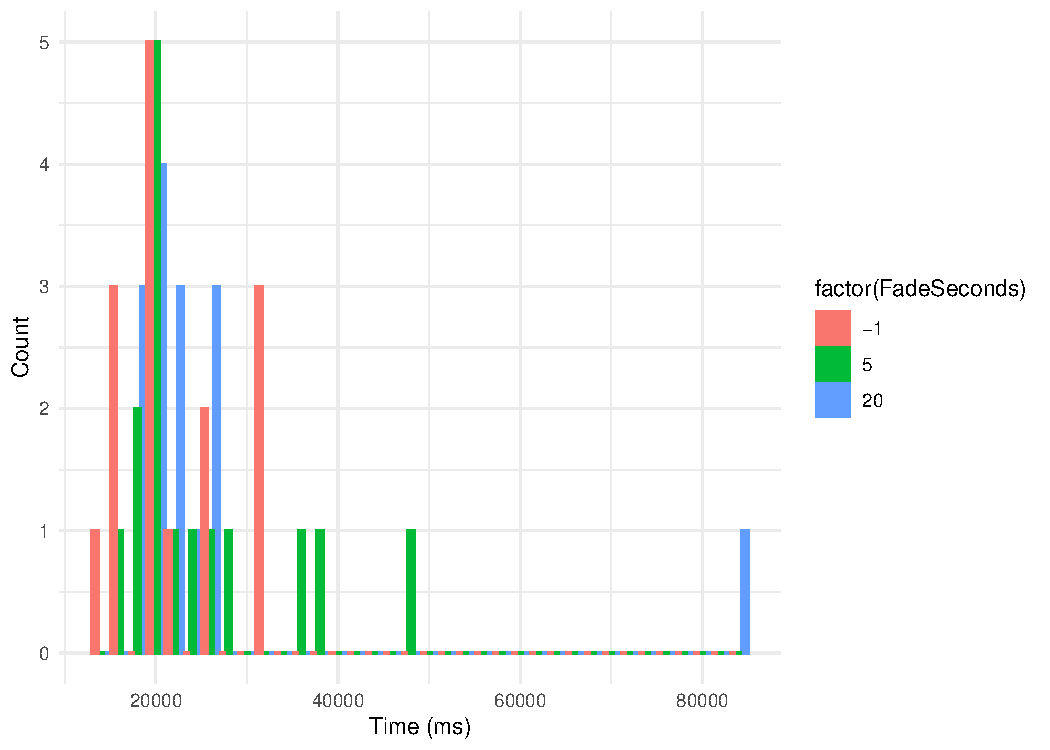
\includegraphics[width=0.75\textwidth]{./_StudyResults/matchingTimeHist}
	\caption{Histogramm der Zeit (ms) unterteilt in Gruppen zur Erledigung von Aufgabe 2: Stroop-Effekt. Darstellungsgenauigkeit: 2000ms}
	\label{fig:matchingTimeHistogram}
\end{figure}

Zum Bearbeiten der letzten Aufgabe wurden durchschnittlich 32.75 Sekunden gebraucht. Der schnellste Proband war in 15.34 Sekunden fertig und der langsamste Teilnehmer hat 54.15 Sekunden zur Absolvierung benötigt. Da die drei Teilaufgaben immer schwerer wurden, wurde im Vergleich immer mehr Zeit benötigt.
Wie in Abbildung~\ref{fig:countingTimeHistogram} einsehbar gibt es kaum Unterschiede der einzelnen Gruppen. Man kann erkennen, dass die Alarm Gruppe wieder etwas früher im Schnitt fertig war. \todoAll{hier mehr beschreiben nachdem vllt die tabelle da ist}

\begin{figure}[H]
	\centering
	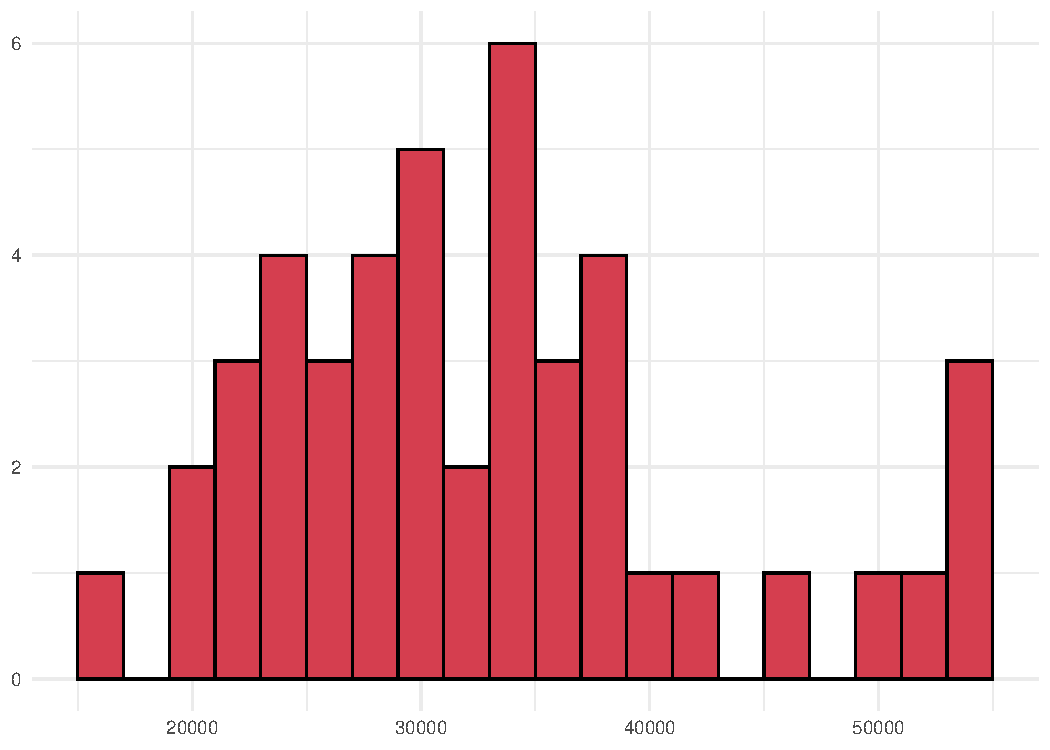
\includegraphics[width=0.75\textwidth]{./_StudyResults/countingTimeHist}
	\caption{Histogramm der Zeit (ms) unterteilt in Gruppen zur Erledigung von Aufgabe 3: Boxen zählen. Darstellungsgenauigkeit: 2000ms}
	\label{fig:countingTimeHistogram}
\end{figure}

Wenn man die Zwischenschritte aus Aufgabe 1 genauer betrachtet, kann man aus Abbildung~\ref{fig:timeTask1} entnehmen, dass nachdem die erste Zahlenblase zerplatzt wurde die zweite Blase innerhalb höchstens 3 Sekunden bei allen Gruppen betätigt wurde. Für die dritte und fünfte Blase ist ein Hochpunkt in allen drei Gruppen erkennbar, was zeigt, dass hier etwas mehr Zeit zur Sortierung benötigt wurde. Ab Zahlenblase sechs waren die Hälfte der Blasen weg, was für ein schnelleres Orientieren sorgt, was sich in den Zeiten wiederspiegelt. Gruppe Fade 5 benötigte im Schnitt etwa 1 Sekunde länger für das Auffinden, der fünften Blase. Darüberhinaus existieren keine großen Unterschiede der einzelnen Studiengruppen.
 
\begin{figure}[H]
	\centering
	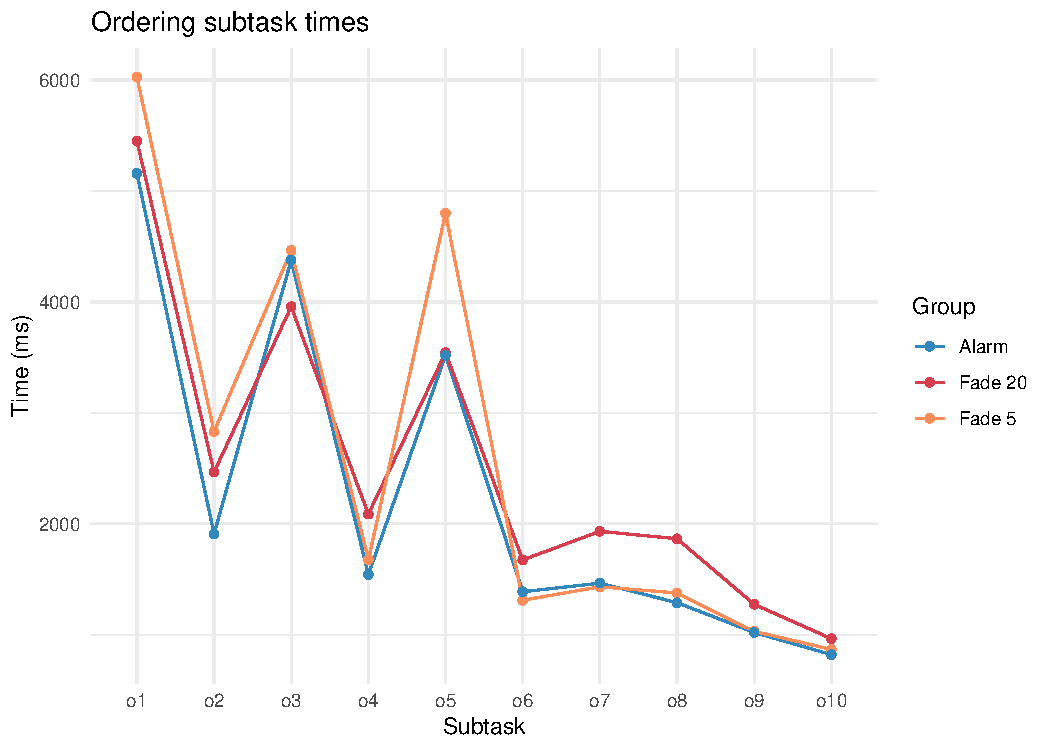
\includegraphics[width=0.75\textwidth]{./_StudyResults/timeTask1}
	\caption{Graph der einzelnen Zeiträume zwischen den Zwischenschritten für Aufgabe 1: Zahlenfolge}
	\label{fig:timeTask1}
\end{figure}

Bei Aufgabe 2 wurden die Zwischenschritte der einzelnen Teilaufgaben ebenso analysiert. In Abbildung~\ref{fig:timeTask2} erkennt man, dass die Fade 5 Gruppe im Schnitt nach 4 Sekunden, also am spätesten im Vergleich, mit Betätigen der ersten Farbblase angefangen hat. Ansonsten bewegen sich die Ergebnisse der drei Gruppen gleichmäßig mit einem Schwankungsbereich von 0.5 Sekunden.

\begin{figure}[H]
	\centering
	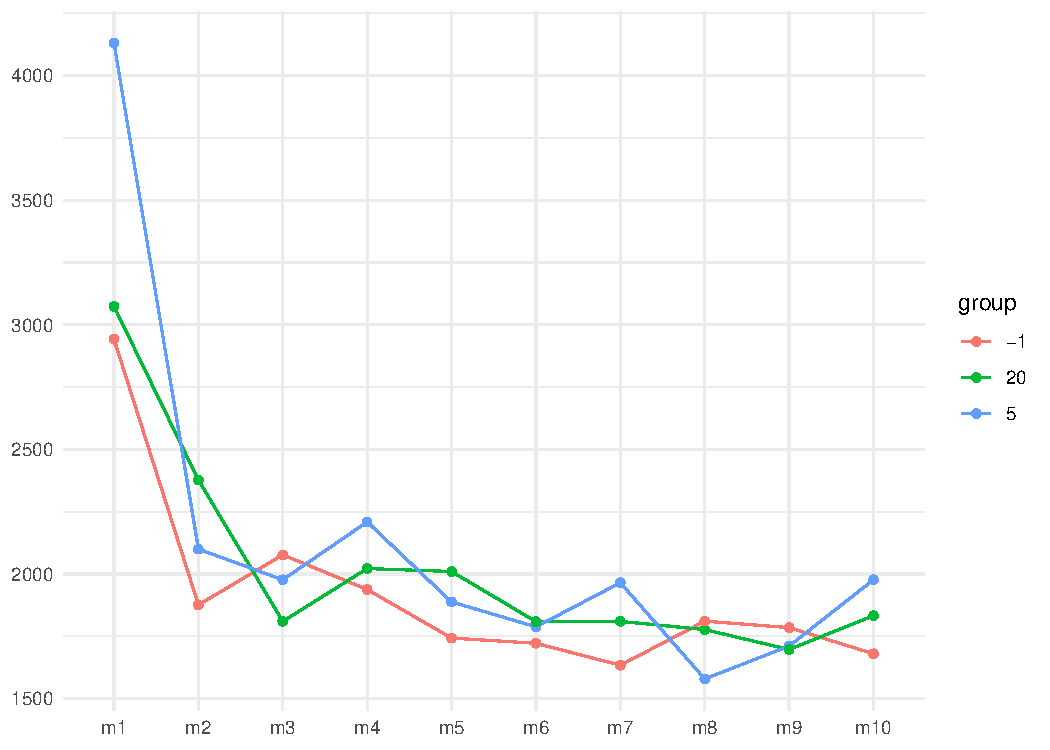
\includegraphics[width=0.75\textwidth]{./_StudyResults/timeTask2}
	\caption{Graph der einzelnen Zeiträume zwischen den Zwischenschritten für Aufgabe 2: Stroop-Effekt}
	\label{fig:timeTask2}
\end{figure}

In der Aufgabe des Boxenzählens wurden ebenso die Zwischenzeiten der Teilaufgaben gemessen wie in Abbildung~\ref{fig:timeTask3} zu sehen ist. Die Alarm Gruppe hat die erste Teilaufgabe am schnellsten beantwortet. Diese Gruppe hat im Schnitt ca 8 Sekunden für die erste Zahlenblase gebraucht und dann kontinuierlich, sogar fast linear länger pro Teilaufgabe gebraucht. Im Gegensatz dazu haben die anderen beiden Gruppen Fade 20 und Fade 5 fast 10 Sekunden für die erste Teilaufgabe gebraucht und verbesserten die Zeit bis zur letzten Betätigung der Zahlenblase. Die Gruppe Fade 20 hat am längsten für die zweite Aufgabe gebraucht aber war dafür am schnellsten bei der letzten Teilaufgabe.

\begin{figure}[H]
	\centering
	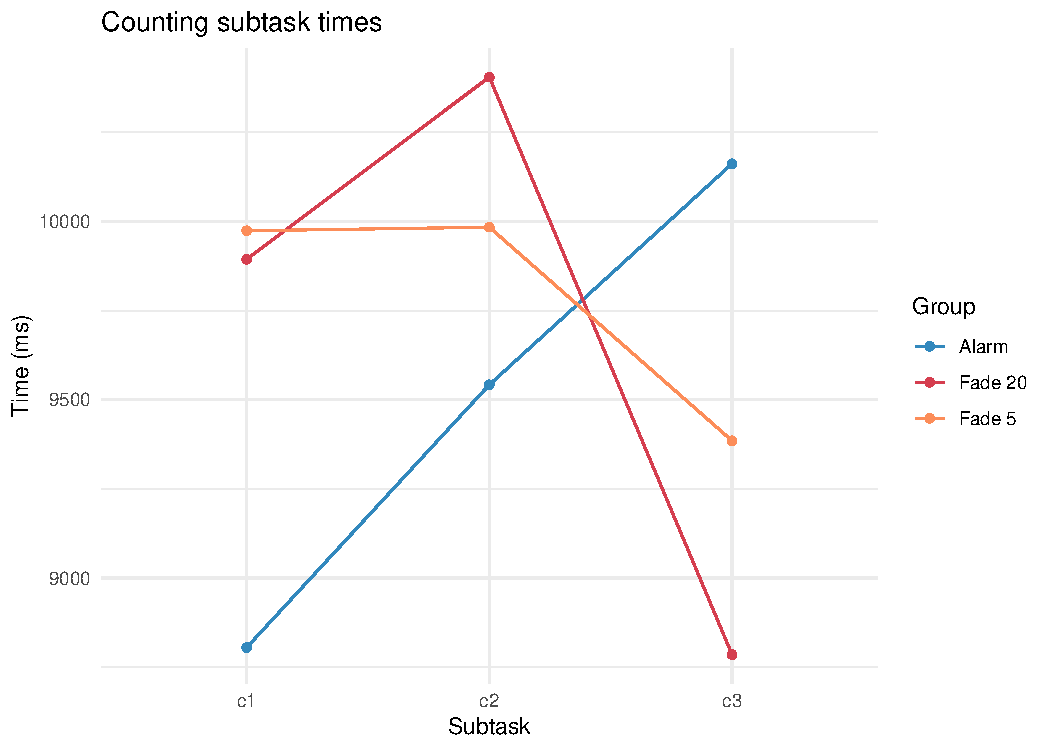
\includegraphics[width=0.75\textwidth]{./_StudyResults/timeTask3}
	\caption{Graph der einzelnen Zeiträume zwischen den Zwischenschritten für Aufgabe 3: Boxen zählen}
	\label{fig:timeTask3}
\end{figure}


\subsection{Selbsteinschätzungen, Fragebögen}\todoAll{subsection ggf umbennen}
%nur Vorschläge zur Gleiderung; hier sowas wie.. SAM, oder so..?

\todoTob{Ergebnisse: Kopfbewegungen}

\todoLuc{Abschnitt zu Ergebnisse von SAM schreiben}
Das Ausfüllen des SAM Fragebogen wurde einmal vor und einmal nach der Ruhephase verlangt. 

\begin{figure}[H]
	\centering
	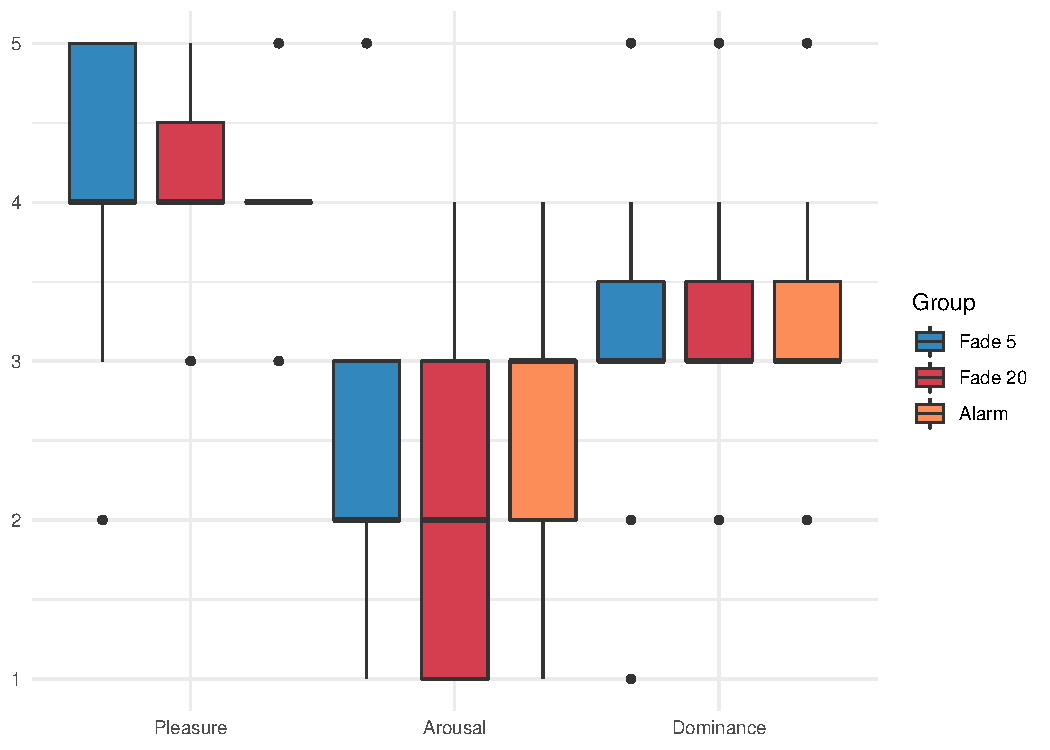
\includegraphics[width=0.75\textwidth]{./_StudyResults/SAMpre}
	\caption{Self-Assessment Manikin Ergebnisse vor der Ruhephase}
	\label{fig:samPre}
\end{figure}
\begin{figure}[H]
	\centering
	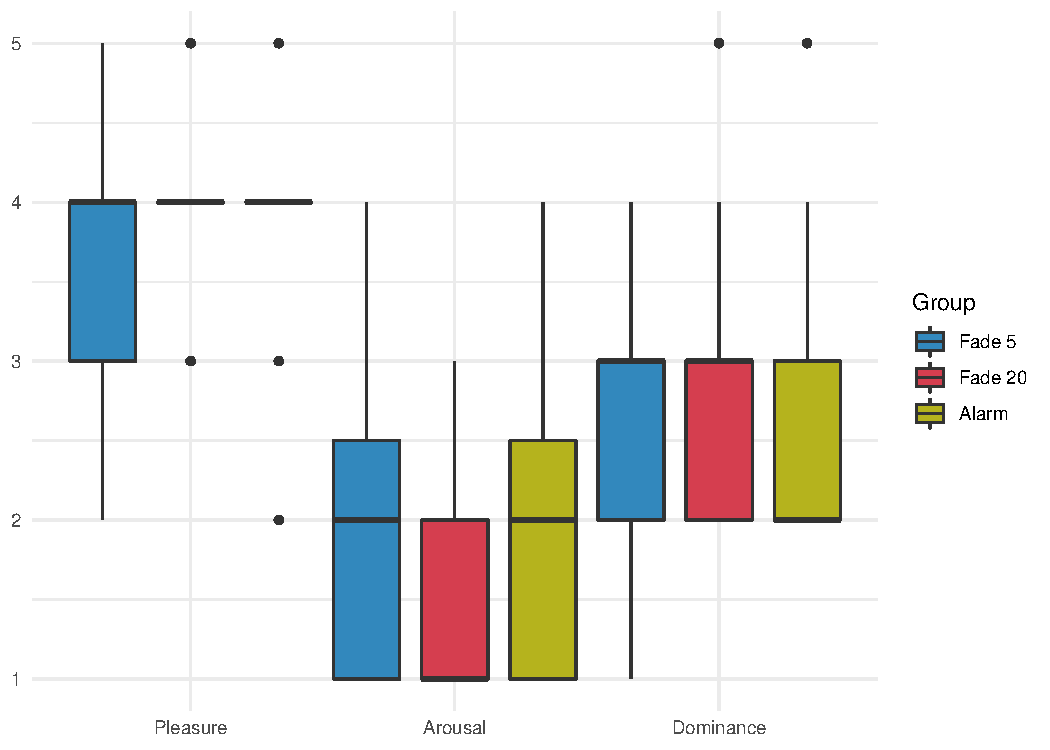
\includegraphics[width=0.75\textwidth]{./_StudyResults/SAMpost}
	\caption{Self-Assessment Manikin Ergebnisse nach der Ruhephase}
	\label{fig:samPost}
\end{figure}


Laut Befragung der Probanden im Anschluss an die Studie haben 20\% geschlafen, beziehungsweise mit den Teilnehmern, die fast geschlafen haben landet man bei 46,7\%. Ein geringer Prozentsatz hat meditiert und die anderen Nutzer gaben an nicht geschlafen zu haben, jedoch waren hier die meisten laut eigener Aussage trotzdem sehr entspannt. Genaue prozentuale Anteile können der Tabelle~\ref{tab:sleepstatus} und Abbildung~\ref{fig:slept} entnommen werden.

\begin{figure}
	\centering
	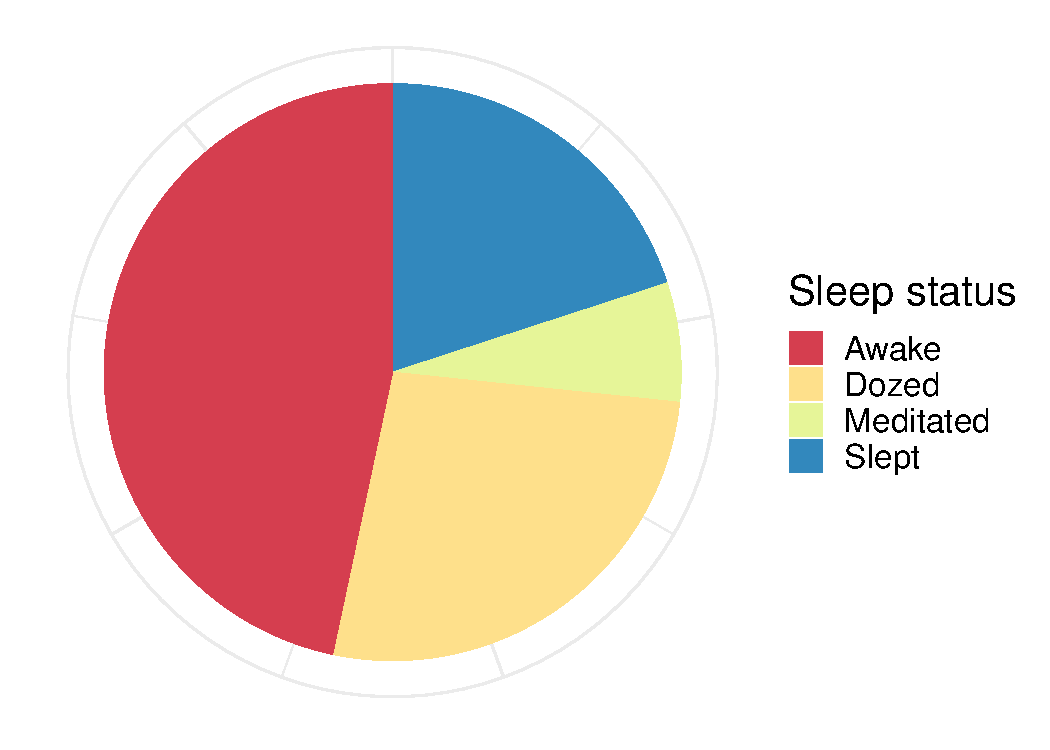
\includegraphics[width=0.75\textwidth]{./_StudyResults/slept}
	\caption{Subjektive Einschätzung der Dauer der Schlafphase}
	\label{fig:slept}
\end{figure}

Die empfundene Schlafdauer variiert in einem Zeitintervall zwischen 8 und 30 Minuten, wobei ein deutlicher Häufungspunkt bei der 15 Minuten Dauer anfällt und die 30 Minuten Angabe ein einzelner Ausreißer ist. Eine genaue Auflistung der Zeitangaben kann in Tabelle~\ref{tab:sleepduration} und Abbildung~\ref{fig:subjectiveSleepDuration} eingesehen werden.

\begin{figure}
	\centering
	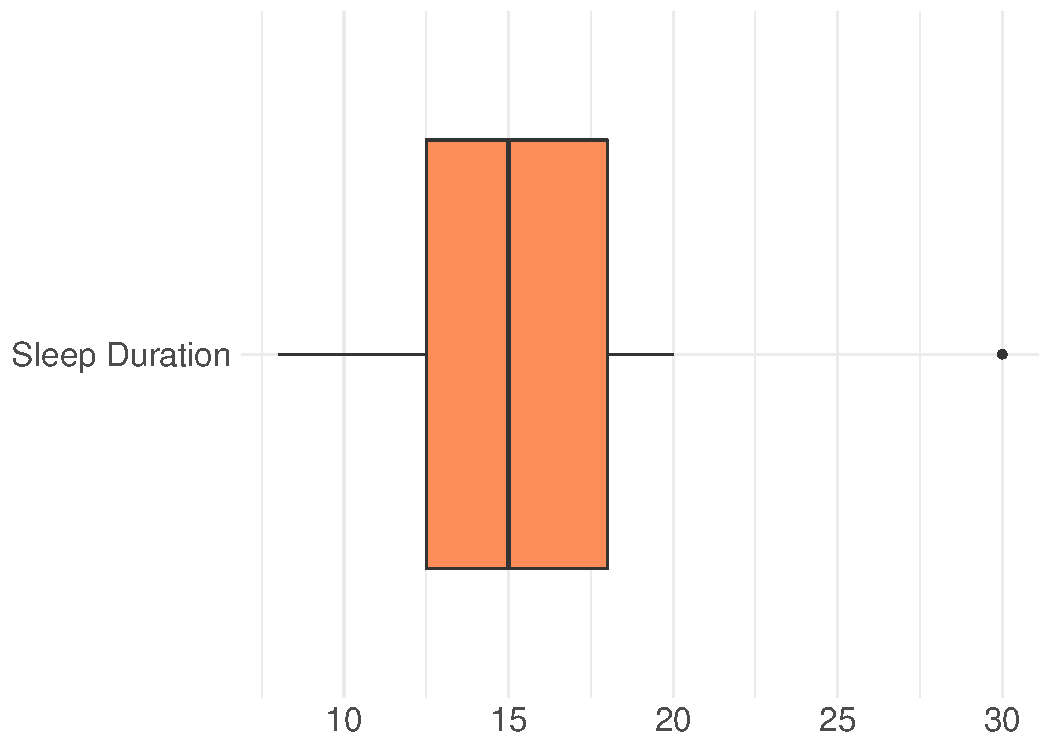
\includegraphics[width=0.75\textwidth]{./_StudyResults/subjectiveSleepDuration}
	\caption{Subjektive Einschätzung der Dauer der Schlafphase}
	\label{fig:subjectiveSleepDuration}
\end{figure}

\begin{figure}
	\centering
	\begin{subfigure}{0.48\textwidth}
		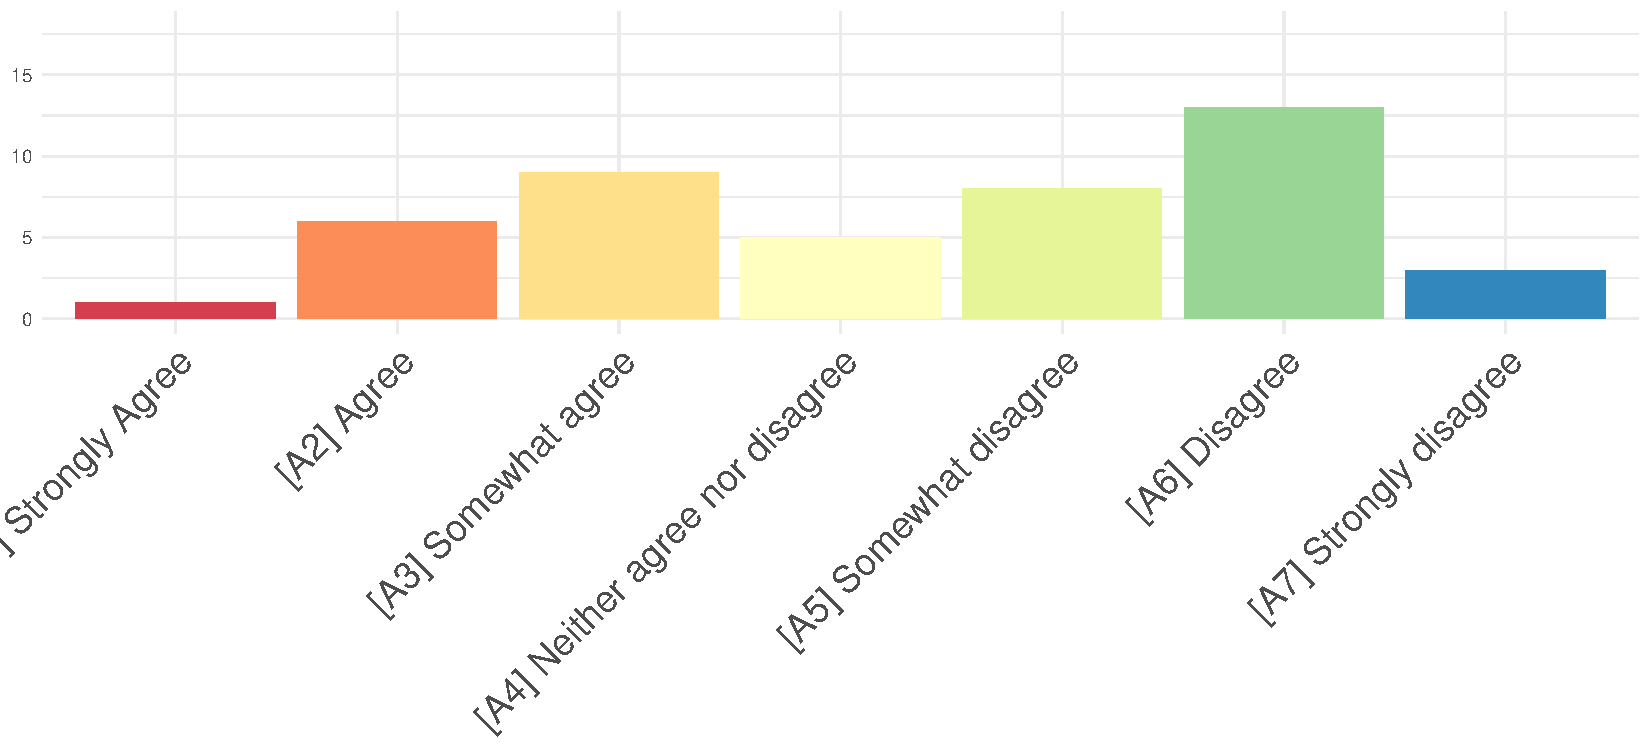
\includegraphics[width=\textwidth]{./_StudyResults/tiredBefore}
		\caption{Tired before}
		\label{fig:tiredBefore}
	\end{subfigure}%
	\hfill
	\begin{subfigure}{0.48\textwidth}
		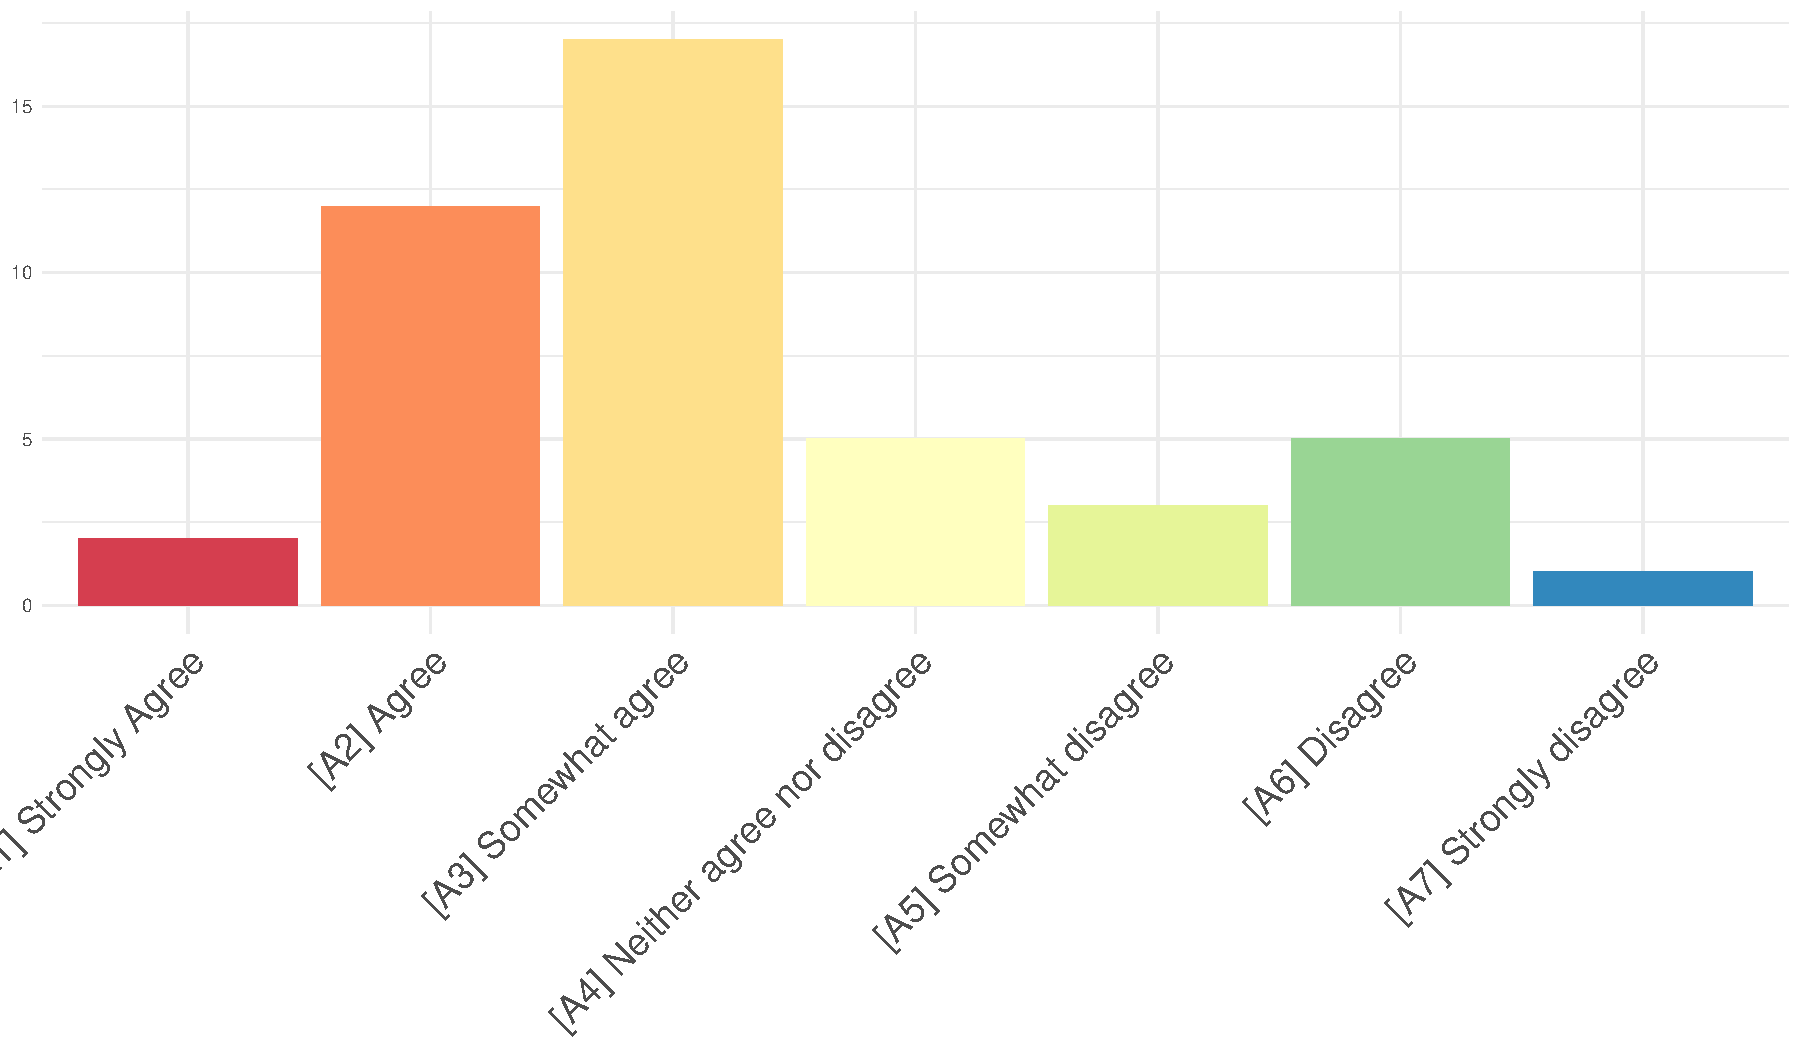
\includegraphics[width=\textwidth]{./_StudyResults/tiredAfter}
		\caption{Tired after}
		\label{fig:tiredAfter}
	\end{subfigure}
	\caption{Tired before and tired after} % caption for whole figure
\end{figure}

\begin{figure}
	\centering
	\begin{subfigure}{0.48\textwidth}
		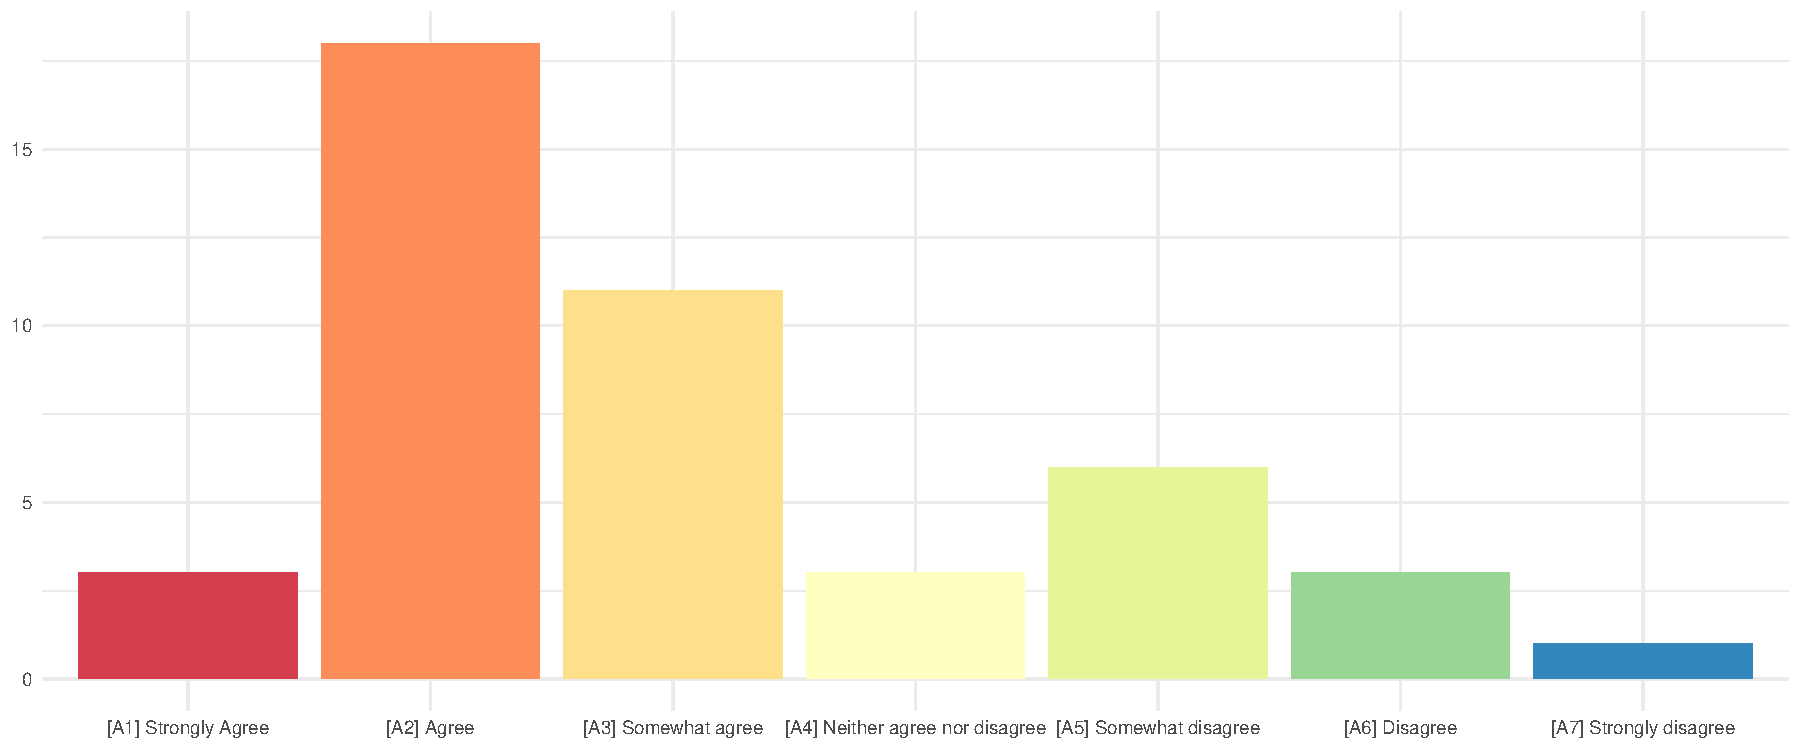
\includegraphics[width=\textwidth]{./_StudyResults/transitionEasy}
		\caption{Transition easy}
		\label{fig:transitionEasy}
	\end{subfigure}%
	\hfill
	\begin{subfigure}{0.48\textwidth}
		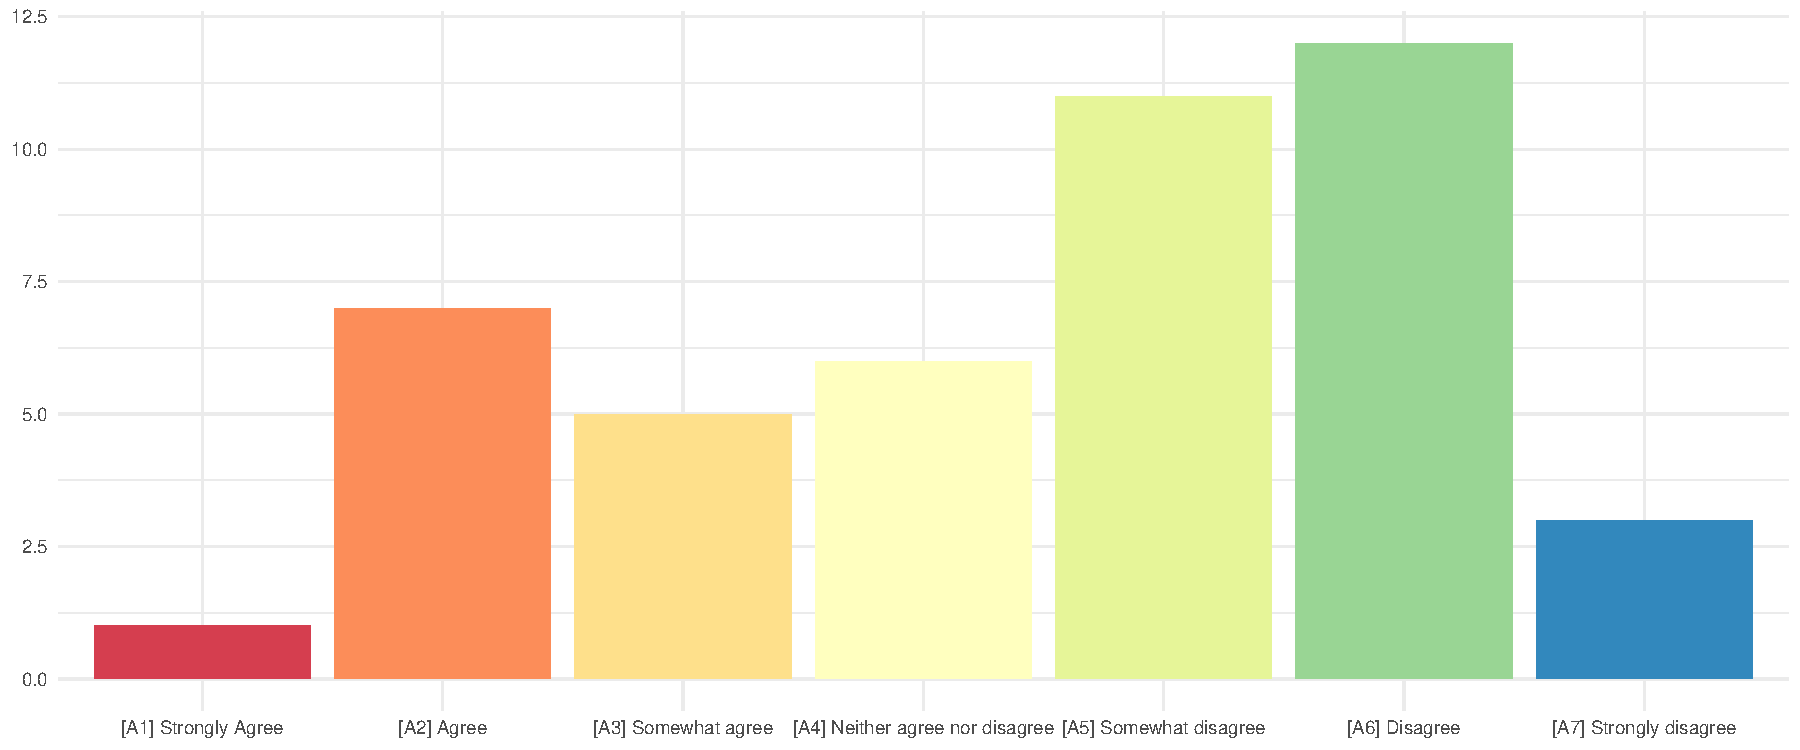
\includegraphics[width=\textwidth]{./_StudyResults/transitionHard}
		\caption{Transition hard}
		\label{fig:transitionHard}
	\end{subfigure}
	\caption{Transitions} % caption for whole figure
\end{figure}

\begin{figure}
	\centering
	\begin{subfigure}{0.48\textwidth}
		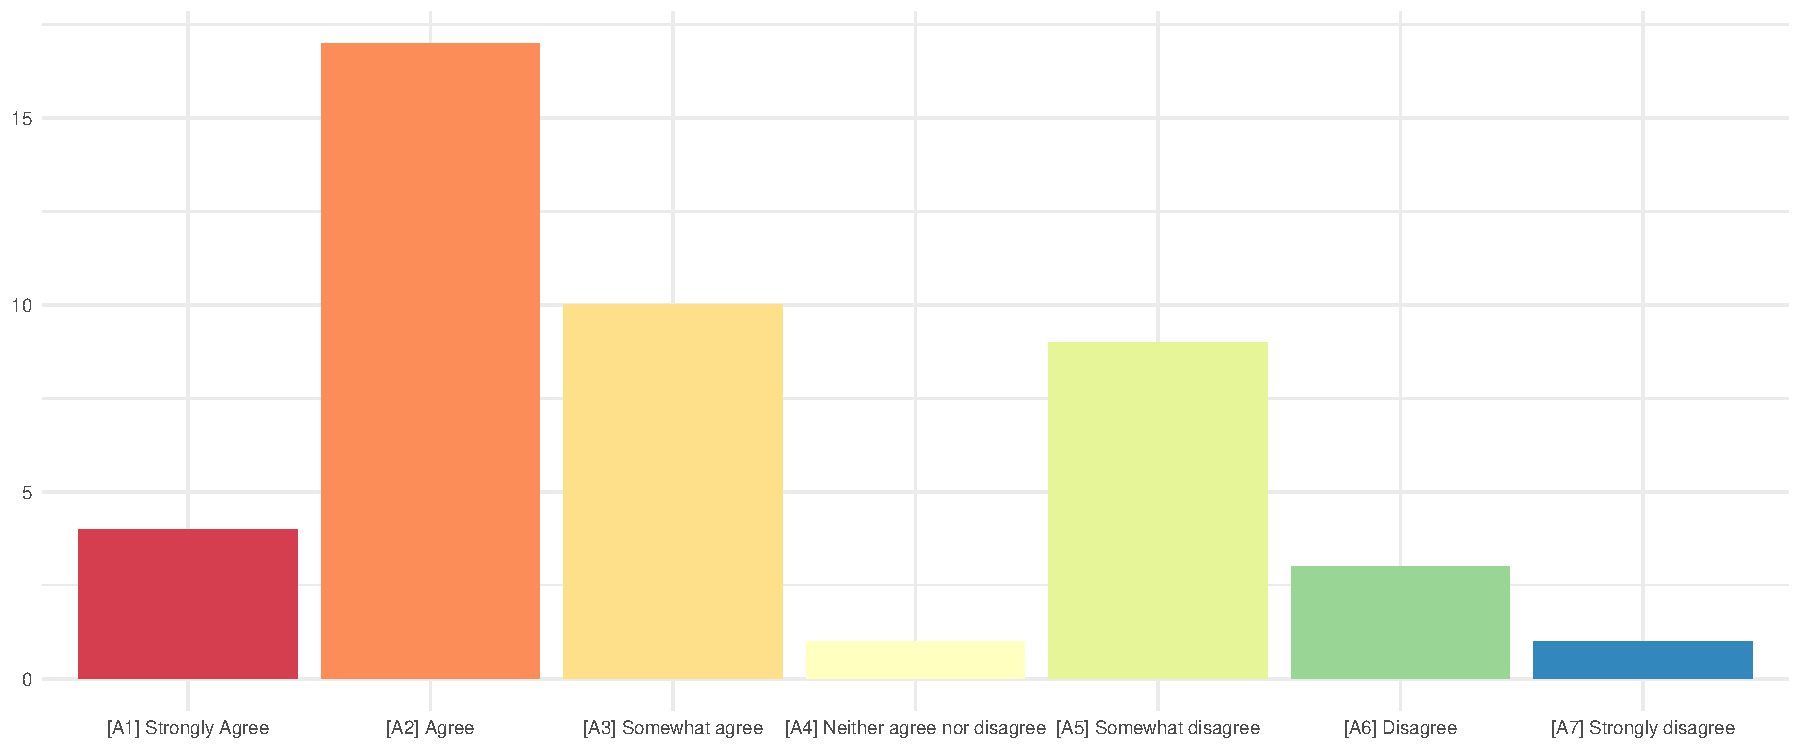
\includegraphics[width=\textwidth]{./_StudyResults/comfortableHeadset}
		\caption{comfortableHeadset}
		\label{fig:comfortableHeadset}
	\end{subfigure}%
	\hfill
	\begin{subfigure}{0.48\textwidth}
		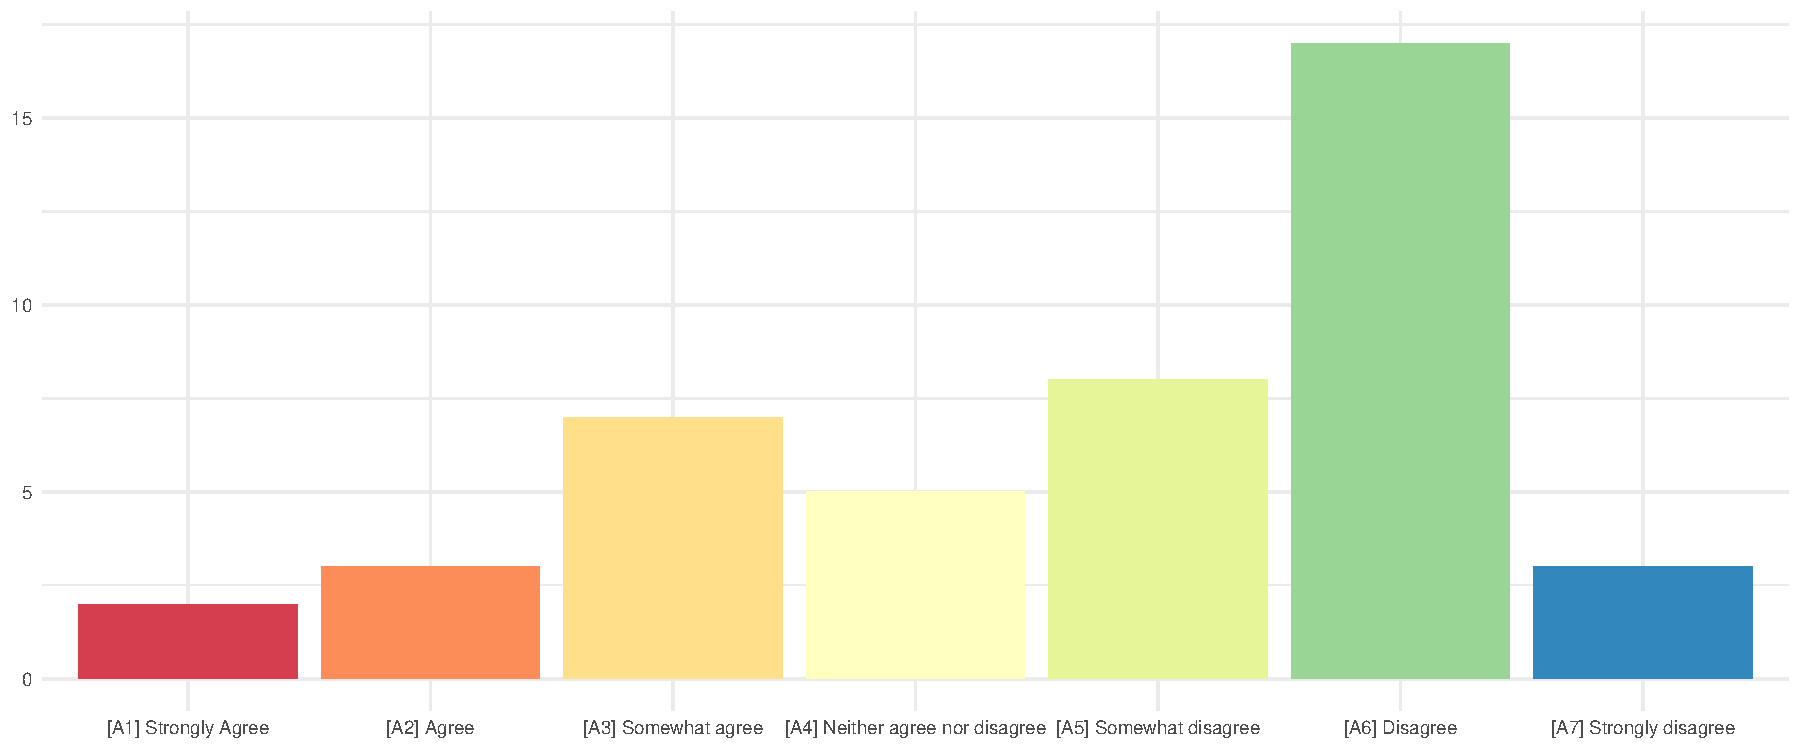
\includegraphics[width=\textwidth]{./_StudyResults/notComfortableHeadset}
		\caption{notComfortableHeadset}
		\label{fig:notComfortableHeadset}
	\end{subfigure}
	\caption{Headset comfort} % caption for whole figure
\end{figure}

\begin{figure}
	\centering
	\begin{subfigure}{0.48\textwidth}
		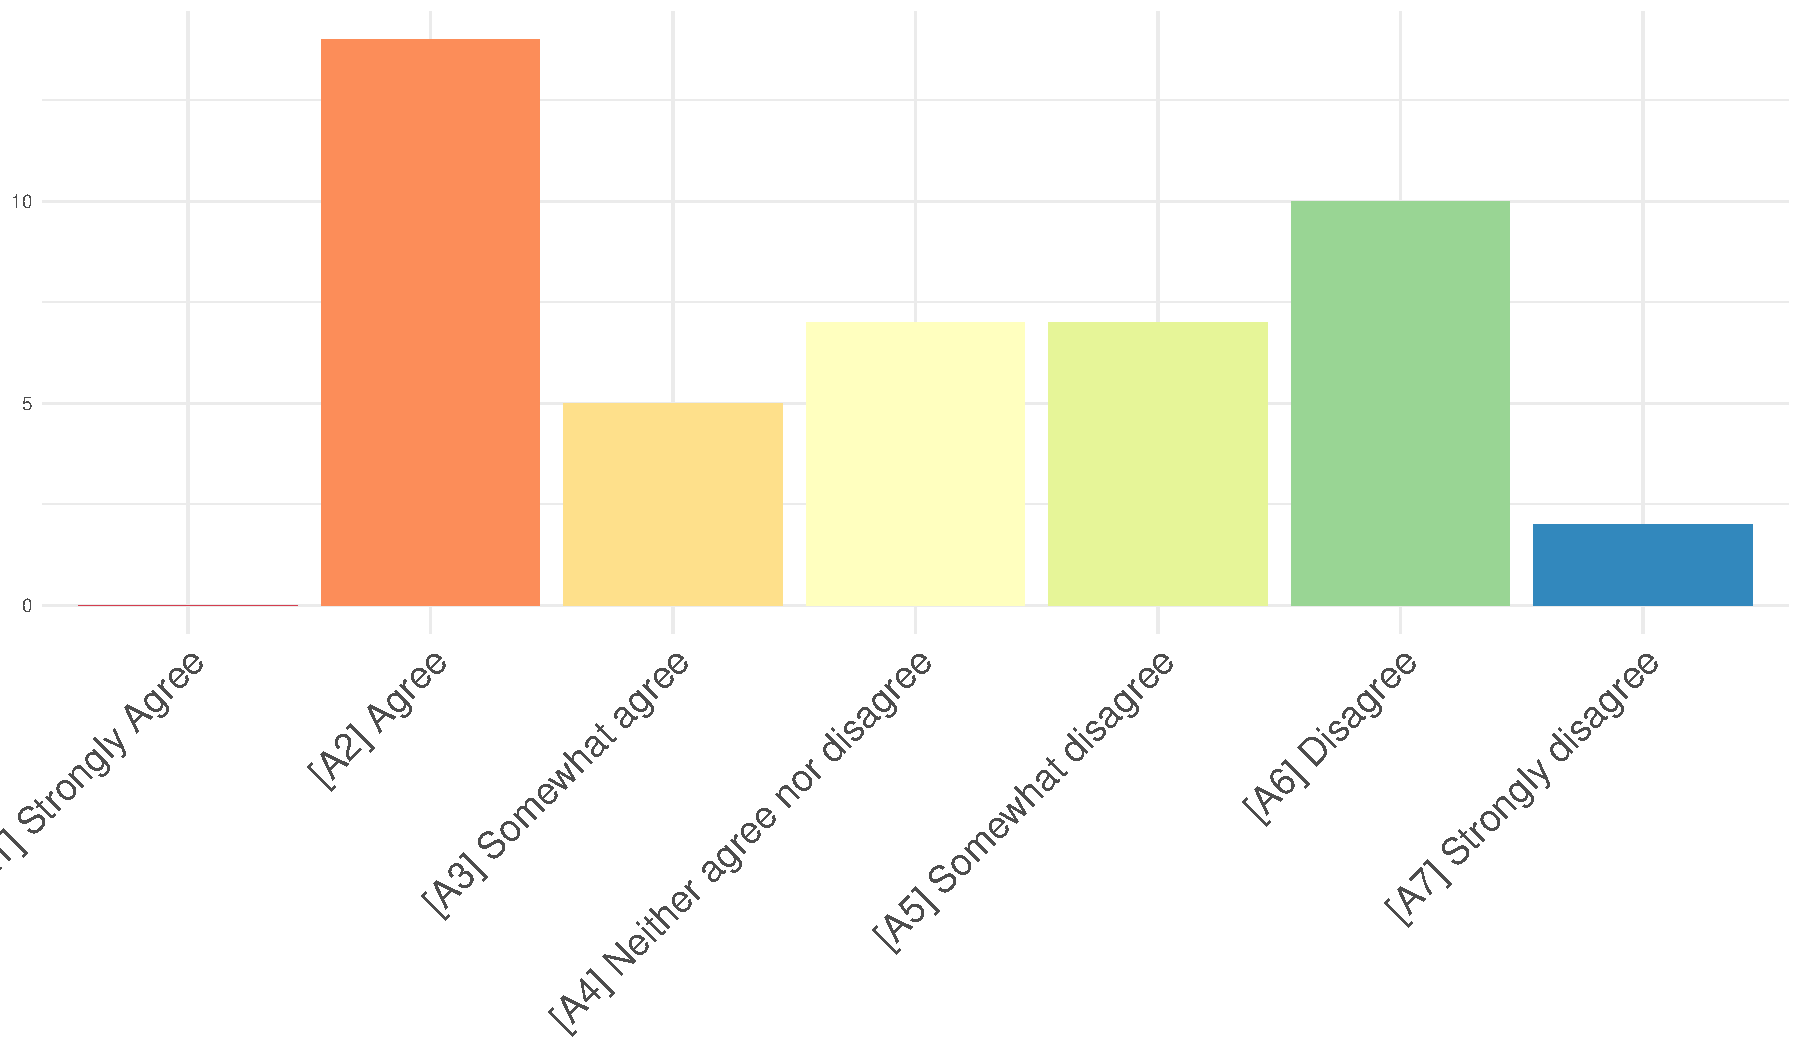
\includegraphics[width=\textwidth]{./_StudyResults/imagineWakingUp}
		\caption{imagineWakingUp}
		\label{fig:imagineWakingUp}
	\end{subfigure}%
	\hfill
	\begin{subfigure}{0.48\textwidth}
		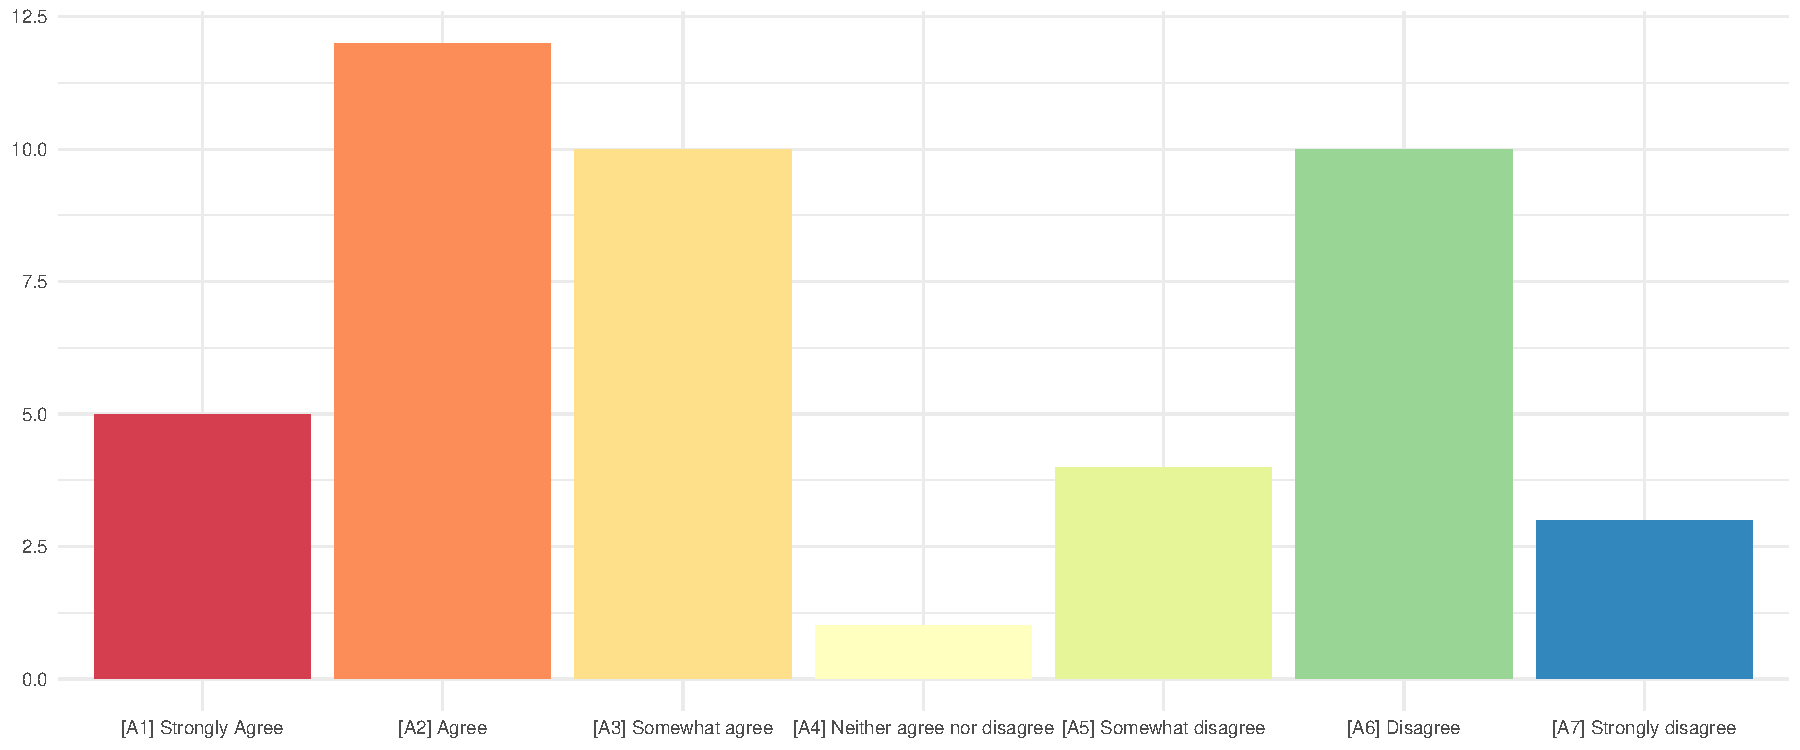
\includegraphics[width=\textwidth]{./_StudyResults/permanentWearing}
		\caption{permanentWearing}
		\label{fig:permanentWearing}
	\end{subfigure}
	\caption{Wearing} % caption for whole figure
\end{figure}

\begin{figure}
	\centering
	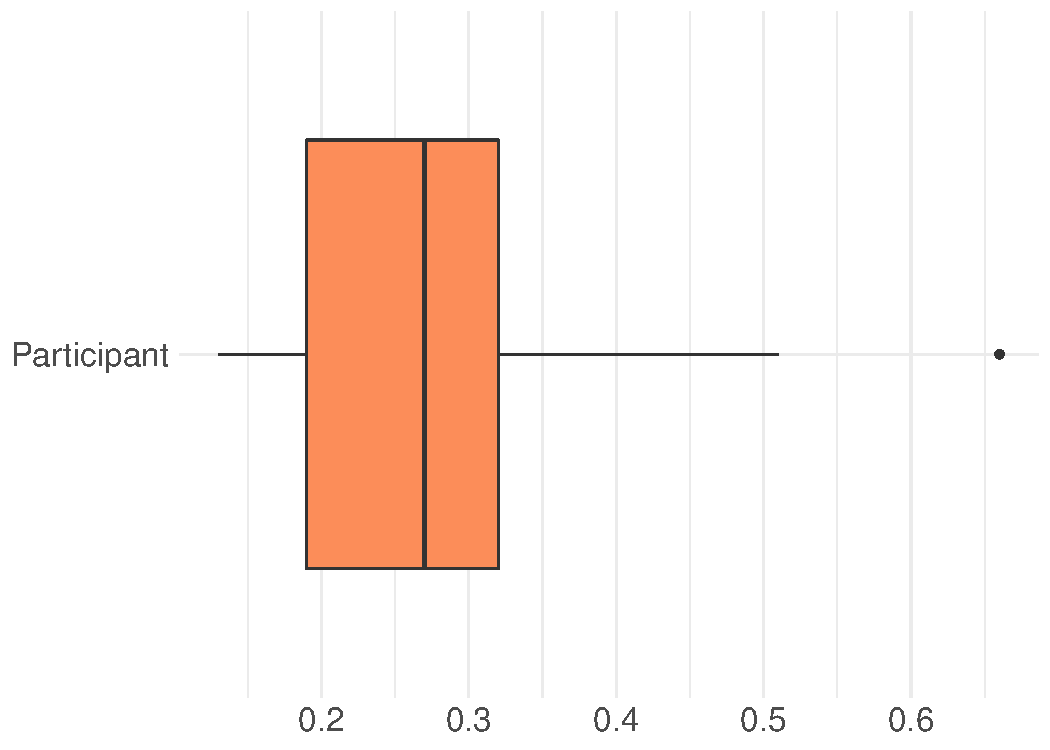
\includegraphics[width=0.75\textwidth]{./_StudyResults/rsme}
	\caption{RSME Visualisierung}
	\label{fig:rsme_vis}
\end{figure}
